\documentclass[11pt,a4paper]{article}
\usepackage{fontspec}
\setmainfont{Arial}
\usepackage[spanish,es-noshorthands,es-tabla]{babel}
\usepackage[a4paper,margin=2.2cm]{geometry}
\usepackage{amsmath,amssymb}
\usepackage{icomma}
\usepackage{graphicx}
\usepackage{booktabs}
\usepackage{array}
\usepackage{multirow}
\usepackage{caption}
\usepackage{float}
\usepackage{enumitem}
\usepackage{tikz}
\usetikzlibrary{arrows.meta,positioning,calc}
\usepackage[backend=biber,style=numeric-comp,sorting=none,maxbibnames=6,url=false,isbn=false,doi=true,eprint=true]{biblatex}
\AtEveryBibitem{\clearfield{issn}\clearlist{language}\clearfield{month}}
\addbibresource{references.bib}
\setcounter{biburlnumpenalty}{9000}\setcounter{biburllcpenalty}{7000}\setcounter{biburlucpenalty}{8000}
\usepackage[hidelinks]{hyperref}
\graphicspath{{figuras/}}
\captionsetup{font=small,labelfont=bf}
\setlength{\parskip}{0.45em}
\setlength{\parindent}{0pt}
\newcommand{\bh}{\hat\beta}
\newcommand{\fwc}{f_{\mathrm{WC}}}
\renewcommand{\arraystretch}{1.12}

\title{Identificación gray-box del modelo de Wilson-Cowan\\con física omitida y su evaluación en lazo cerrado}
\author{}
\date{}

\begin{document}
\maketitle
\vspace{-14mm}

\begin{abstract}
\noindent Los controladores basados en modelo para la regulación optogenética de la actividad neuronal usan versiones reducidas del modelo de Wilson-Cowan, que omiten parte de la física de la planta. Se estudió la identificación de modelos gray-box de Wilson-Cowan a partir de datos sintéticos con ruido de medición, generados por un simulador que agrega un mecanismo omitido por vez, el factor refractario o un actuador con un filtro de primer orden de 1~ms y un recorte en $\pm 3$. Se compararon cuatro familias de modelos con el mismo backbone de Wilson-Cowan: el white-box, las correcciones con red neuronal (agnóstica, con historia del comando y con filtro entrenable), el backbone expandido, que agrega la ecuación del mecanismo omitido con parámetros físicos entrenables, y una referencia black-box. Cada modelo se evaluó en lazo abierto, por su reproducción de estímulos no vistos y por la recuperación de los parámetros, y en lazo cerrado, como planta del controlador IMC de Martínez et al.\ sin modificar. Se usaron dos regímenes de datos, con comandos en $[0, 2]$ y con comandos bipolares de hasta $\pm 12$. En la planta refractaria, la corrección agnóstica con arranque desde el white-box identificó los parámetros con 3,5~\% de error medio con comandos en $[0, 2]$, y con 1,7~\% con comandos de amplitud grande. En la planta con actuador, solo el backbone expandido recuperó los parámetros (0,1 a 0,5~\% con $\sigma = 0{,}01$), y con comandos de amplitud grande identificó también el nivel del recorte (2,99 a 3,01). Las correcciones con historia del comando y con filtro entrenable mejoraron la reproducción en lazo abierto con parámetros alejados de los verdaderos (errores de 18,6 a 210~\%). Con comandos en $[0, 2]$, en lazo cerrado quedaron más lejos del lazo con el simulador que el white-box, que reproducía peor en lazo abierto. El error de seguimiento de la referencia no ordenó a los modelos según su parecido con la planta en lazo cerrado. Con ruido de medición, iniciar cada ventana de entrenamiento desde el estado medido sesgó los parámetros, y un estado inicial entrenable por ventana lo corrigió en el white-box sobre la planta ideal y en el backbone expandido con actuador.
\end{abstract}

\tableofcontents
\newpage

%=====================================================================
\section{Introducción}
%=====================================================================

\subsection{Contexto}

El control optogenético en lazo cerrado busca llevar la actividad de una población neuronal a un patrón prescrito, ajustando la luz en tiempo real \cite{grosenick2015,newman2015,zaaimi2023}. Los controladores basados en modelo necesitan una descripción de cómo responde la población al comando. Las ecuaciones de Wilson-Cowan son una elección habitual \cite{wilson1972,chow2020}, porque describen la actividad media de poblaciones excitatorias e inhibitorias acopladas con pocos parámetros interpretables. Sobre este modelo se propusieron controladores para regular actividad oscilatoria, como el control por modelo interno (IMC) de patrones theta-gamma de Martínez et al.\ \cite{martinez2022ifac} y modelos lineales de parámetros variables de la población actuada \cite{martinez2024lpv}.

\subsection{Planteo del problema}

El modelo reducido que usa el controlador omite parte de la física de la planta. El factor refractario de la formulación original suele quitarse \cite{kilpatrick2013,chow2020,martinez2022ifac}, con la justificación de que equivale a reescalar la sigmoidea \cite{kilpatrick2013}. Ese factor escala la respuesta por un término que depende de la actividad, así que las dos formas difieren cuando la actividad es alta. Los modelos que tratan la refractariedad como un estado aparte muestran además otros comportamientos, como oscilaciones en una sola población excitatoria \cite{painchaud2022,weistuch2020}. La planta de este trabajo conserva la forma cuasi estática del modelo original.

El actuador optogenético se supone ideal en los diseños basados en modelo \cite{martinez2022ifac}. En la práctica la opsina filtra el comando como un pasabajos \cite{williams2013,tchumatchenko2013}, y la luz que se puede entregar está acotada \cite{newman2015}. Un controlador diseñado sobre el modelo reducido actúa entonces sobre una planta distinta de su descripción interna. Para diseñar y probar en simulación estos controladores hace falta un modelo que reproduzca la planta, incluidos los términos omitidos.

\subsection{Antecedentes}

Los modelos gray-box combinan un backbone mecanístico con una componente entrenable que representa lo que el mecanismo deja afuera \cite{psichogios1992,rackauckas2020}. Con ecuaciones diferenciales ordinarias neuronales (Neural ODE) \cite{chen2018}, la corrección es una red dentro del campo vectorial, y los parámetros del backbone se estiman junto con los pesos de la red \cite{yin2021,giampiccolo2024}. Un modelo de tasas del tipo Wilson-Cowan se escribió de esta forma, con una red para la dinámica estocástica no modelada \cite{elgazzar2025}, y modelos híbridos de este tipo se usaron para identificar ecuaciones de orden reducido de poblaciones neuronales \cite{chesebro2025}. Los parámetros del backbone conservan su significado físico.

Tres aspectos hacen difícil el problema. El primero es que la física omitida puede tener memoria propia. El término refractario depende del estado actual, mientras que el actuador agrega un estado oculto que depende del comando pasado. Una corrección que recibe solo el estado observado no puede representar el segundo caso, y la arquitectura de la corrección tiene que acompañar el tipo de física faltante, con memoria del comando \cite{forgione2021} o con un estado aumentado \cite{dupont2019}. El segundo es que el esquema de entrenamiento puede sesgar las estimaciones. El multiple shooting parte registros largos en ventanas cortas \cite{ribeiro2020,turan2022}, y arrancar cada ventana desde el estado medido se considera inadecuado con datos ruidosos \cite{turan2022}, porque el ruido entra en las condiciones iniciales. Los codificadores que estiman el estado inicial de cada ventana a partir de datos pasados son una alternativa \cite{beintema2021}. El tercero es que la precisión predictiva no garantiza utilidad para el control. Un modelo es adecuado para el control cuando el lazo cerrado construido con el modelo se parece al construido con la planta \cite{gevers2005}, y la precisión predictiva de un modelo y el desempeño del controlador basado en él pueden no coincidir \cite{lambert2020,bolus2018}. Además, los modelos identificados no deberían usarse fuera del rango de los datos de identificación \cite{schoukens2019}, y un controlador puede llevar al modelo fuera de ese rango.

\subsection{Objetivos e hipótesis}

El objetivo general fue obtener modelos de Wilson-Cowan entrenados con datos ruidosos de una planta con física omitida que se comporten como esa planta en lazo abierto y en lazo cerrado. Los objetivos específicos fueron los siguientes.

\begin{enumerate}[leftmargin=*,itemsep=0.2em]
\item Comparar arquitecturas de corrección gray-box frente a dos mecanismos omitidos de distinta naturaleza, uno sin memoria propia y otro con un estado oculto.
\item Medir la reproducción en lazo abierto de estímulos no vistos, la recuperación de los parámetros del backbone y la reconstrucción del término omitido.
\item Usar cada modelo identificado como planta del controlador IMC de \cite{martinez2022ifac}, sin modificar el controlador, y comparar ese lazo con el lazo sobre el simulador.
\item Cuantificar el sesgo que introduce el esquema de entrenamiento por ventanas con ruido de medición.
\item Evaluar el efecto del rango de los comandos de entrenamiento, comparando datos en el rango que se venía usando con datos en el rango que pide el controlador.
\end{enumerate}

Las hipótesis de trabajo fueron tres. La primera es que la memoria de la física omitida decide qué corrección alcanza. Un término que depende solo del estado lo captura una red del estado, y uno con estado propio requiere memoria del comando o expandir el backbone. La segunda es que reproducir bien en lazo abierto no asegura un lazo cerrado parecido al de la planta. La tercera es que arrancar cada ventana desde el estado medido con ruido sesga los parámetros, y que un estado inicial entrenable lo corrige.

\subsection{Alcance}

El estudio se restringe a datos sintéticos, a un solo controlador y a una perturbación por vez. Las simulaciones de lazo cerrado usan mediciones sin ruido. Las perturbaciones pertenecen a una línea de diseño, con valores elegidos para poner a prueba las arquitecturas de corrección, y el actuador de 1~ms es más rápido que la channelrodopsina-2 \cite{williams2013,tchumatchenko2013}.

%=====================================================================
\section{Métodos}
%=====================================================================

\subsection{Modelo de Wilson-Cowan y plantas simuladas}

El estado es $x = (I, E)^\top$, la actividad de las poblaciones inhibitoria y excitatoria, y la entrada es $u = (P, Q)^\top$, el comando sobre la población excitatoria ($P$) y sobre la inhibitoria ($Q$). Todos los modelos comparten el campo de Wilson-Cowan reducido de \cite{martinez2022ifac},
\begin{equation}
\fwc(x, u; \beta) =
\begin{bmatrix}
\tfrac{1}{\tau_i}\big(-I + \sigma(a_i u_i) - k_i\big)\\[3pt]
\tfrac{1}{\tau_e}\big(-E + \sigma(a_e u_e) - k_e\big)
\end{bmatrix},\qquad
\begin{aligned}
u_i &= w_{IE}E - w_{II}I + Q - \theta_i,\\
u_e &= w_{EE}E - w_{EI}I + P - \theta_e,
\end{aligned}
\label{eq:wc}
\end{equation}
con $\sigma(z) = 1/(1 + e^{-z})$ y los diez parámetros $\beta = (w_{EE}, w_{EI}, w_{IE}, w_{II}, \tau_e, \tau_i, a_e, a_i, \theta_e, \theta_i)$. Los offsets $k_e = \sigma(-a_e\theta_e)$ y $k_i = \sigma(-a_i\theta_i)$ hacen de $E = I = 0$ un equilibrio con $u = 0$, y se recalculan cuando cambian $a$ y $\theta$. El tiempo se mide en milisegundos. Los parámetros verdaderos son los del archivo del controlador de \cite{martinez2022ifac} y figuran en el Apéndice~\ref{ap:parametros}.

Las plantas simuladas agregan a \eqref{eq:wc} un mecanismo que los modelos no tienen.

\textbf{Planta refractaria.} La sigmoidea de cada población se multiplica por $(1 - r\,x_j)$, con $r = 0{,}10$,
\begin{equation}
\tau_j\,\dot x_j = -x_j + (1 - r\,x_j)\,\sigma(a_j u_j) - k_j, \qquad j \in \{i, e\}.
\label{eq:refrac}
\end{equation}

\textbf{Planta con actuador.} A las poblaciones llega la versión filtrada y recortada del comando,
\begin{equation}
\tau\,\dot P_f = P - P_f, \qquad P_{ef} = \min\big(3,\ \max(-3,\ P_f)\big), \qquad \tau = 1~\text{ms},
\label{eq:actuador}
\end{equation}
y lo mismo para $Q$. El recorte es simétrico porque el comando del controlador puede tomar los dos signos. Una versión anterior del actuador usaba la saturación $3\tanh(P_f/3)$, que comprime el comando aun por debajo del nivel (un comando de 2 sale como 1,75). Esa línea se usó en tres tandas de este informe (e16, e19 y e20) y se indica en cada caso (Fig.~\ref{fig:saturacion}).

\textbf{Planta ideal.} El modelo \eqref{eq:wc} sin agregados, usado como referencia del sesgo del entrenamiento.

El término omitido es la diferencia entre el campo de la planta y el backbone con los parámetros verdaderos, $\Delta f = f_{\text{planta}} - \fwc(x, u; \beta)$, evaluada sobre la trayectoria. Solo existe con datos sintéticos, y se guarda junto a cada dataset. En algunas figuras aparece como término faltante.

\begin{figure}[H]
\centering
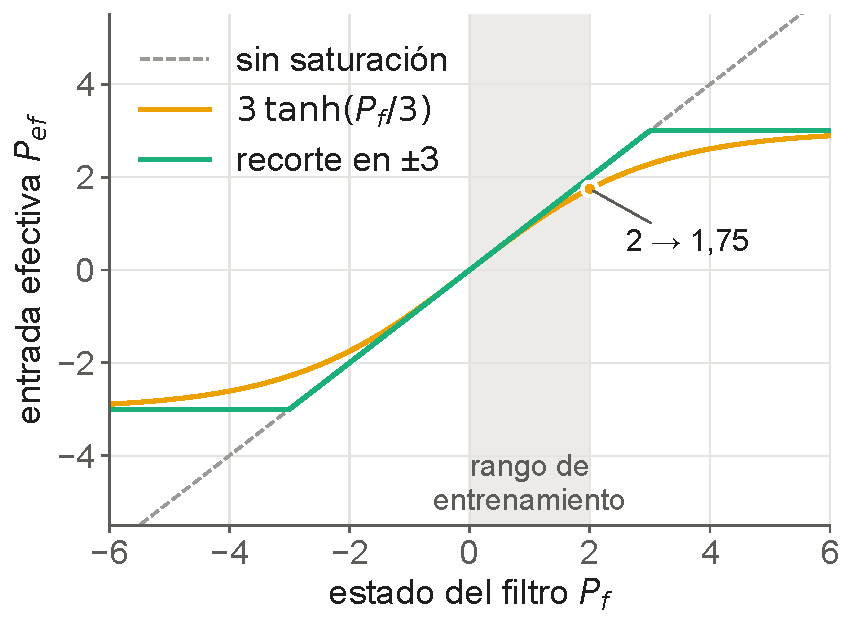
\includegraphics[width=0.55\textwidth]{saturacion.pdf}
\caption{Entrada efectiva $P_{ef}$ en función del estado del filtro $P_f$ para la saturación $3\tanh(P_f/3)$ y para el recorte en $\pm 3$. La franja gris es el rango de comandos de los datos de entrenamiento con amplitud chica.}
\label{fig:saturacion}
\end{figure}

\subsection{Datos}

Cada escenario dura 2~s y se muestrea a 2~kHz ($\Delta t = 0{,}5$~ms, 4001 muestras), con el estímulo encendido entre 100 y 1900~ms. La planta se integra con Runge-Kutta de cuarto orden (RK4) a 0,05~ms, y el comando se mantiene constante entre muestras. A $I$ y $E$ se les suma ruido blanco gaussiano independiente con desvío por muestra de 0,0032 y 0,016. Esos niveles se nombran $\sigma = 0{,}01$ y $\sigma = 0{,}05$, su equivalente con muestreo de 20~kHz, porque el desvío se escala por $\sqrt{2/20}$ para conservar la densidad espectral del ruido. Cada nivel de ruido tiene tres realizaciones (semillas 0, 1 y 2). No se aplica suavizado a los datos.

\textbf{Régimen de amplitud chica.} Siete familias de estímulos on/off: escalón, onda cuadrada, APRBS, PRBS, theta-gamma, tren de Poisson y chirp, con $P$ y $Q$ descorrelacionados. Los comandos cubren $P \in [0, 2]$ y $Q \in [0; 1{,}5]$. Son 49 escenarios: 28 de entrenamiento, 7 de validación (uno por familia) y 14 de test. De los 14 de test, 13 interpolan y uno (un escalón de amplitud 1,2) extrapola en amplitud.

\textbf{Régimen de amplitud grande.} El controlador pide comandos entre $-14$ y $13$ en $P$ y entre $-16$ y $15$ en $Q$ (Sección~\ref{sec:lc_chica}), fuera del rango anterior. Los datasets de este régimen tienen seis familias: onda cuadrada, APRBS, theta-gamma, Poisson, chirp y ruido blanco gaussiano de banda limitada (50, 150 o 400~Hz, con desvío de un tercio de la amplitud y sin recortar). Cada familia aparece con una amplitud por escenario, de 1 a 12 en pasos de 1, y todas son bipolares. Con amplitud $A$, $P$ va de $-A$ a $A$ y $Q$ de $-\tfrac{14}{12}A$ a $\tfrac{14}{12}A$. Son 72 escenarios de entrenamiento, 12 de validación y 26 de test. Validación y test usan amplitudes fuera de la grilla, entre 1,5 y 11,5, y el test incluye además los 14 escenarios de test del régimen anterior sin cambios (Fig.~\ref{fig:ejemplos}).

En el entrenamiento del actuador con amplitud grande, el recorte actúa en el 34~\% de las muestras de $P$ y en el 39~\% de las de $Q$, y el valor eficaz del término omitido en $E$ pasa de 0,034 a 0,241. En la planta refractaria pasa de 0,013 a 0,036 en $E$ y de 0,002 a 0,014 en $I$.

\begin{figure}[H]
\centering
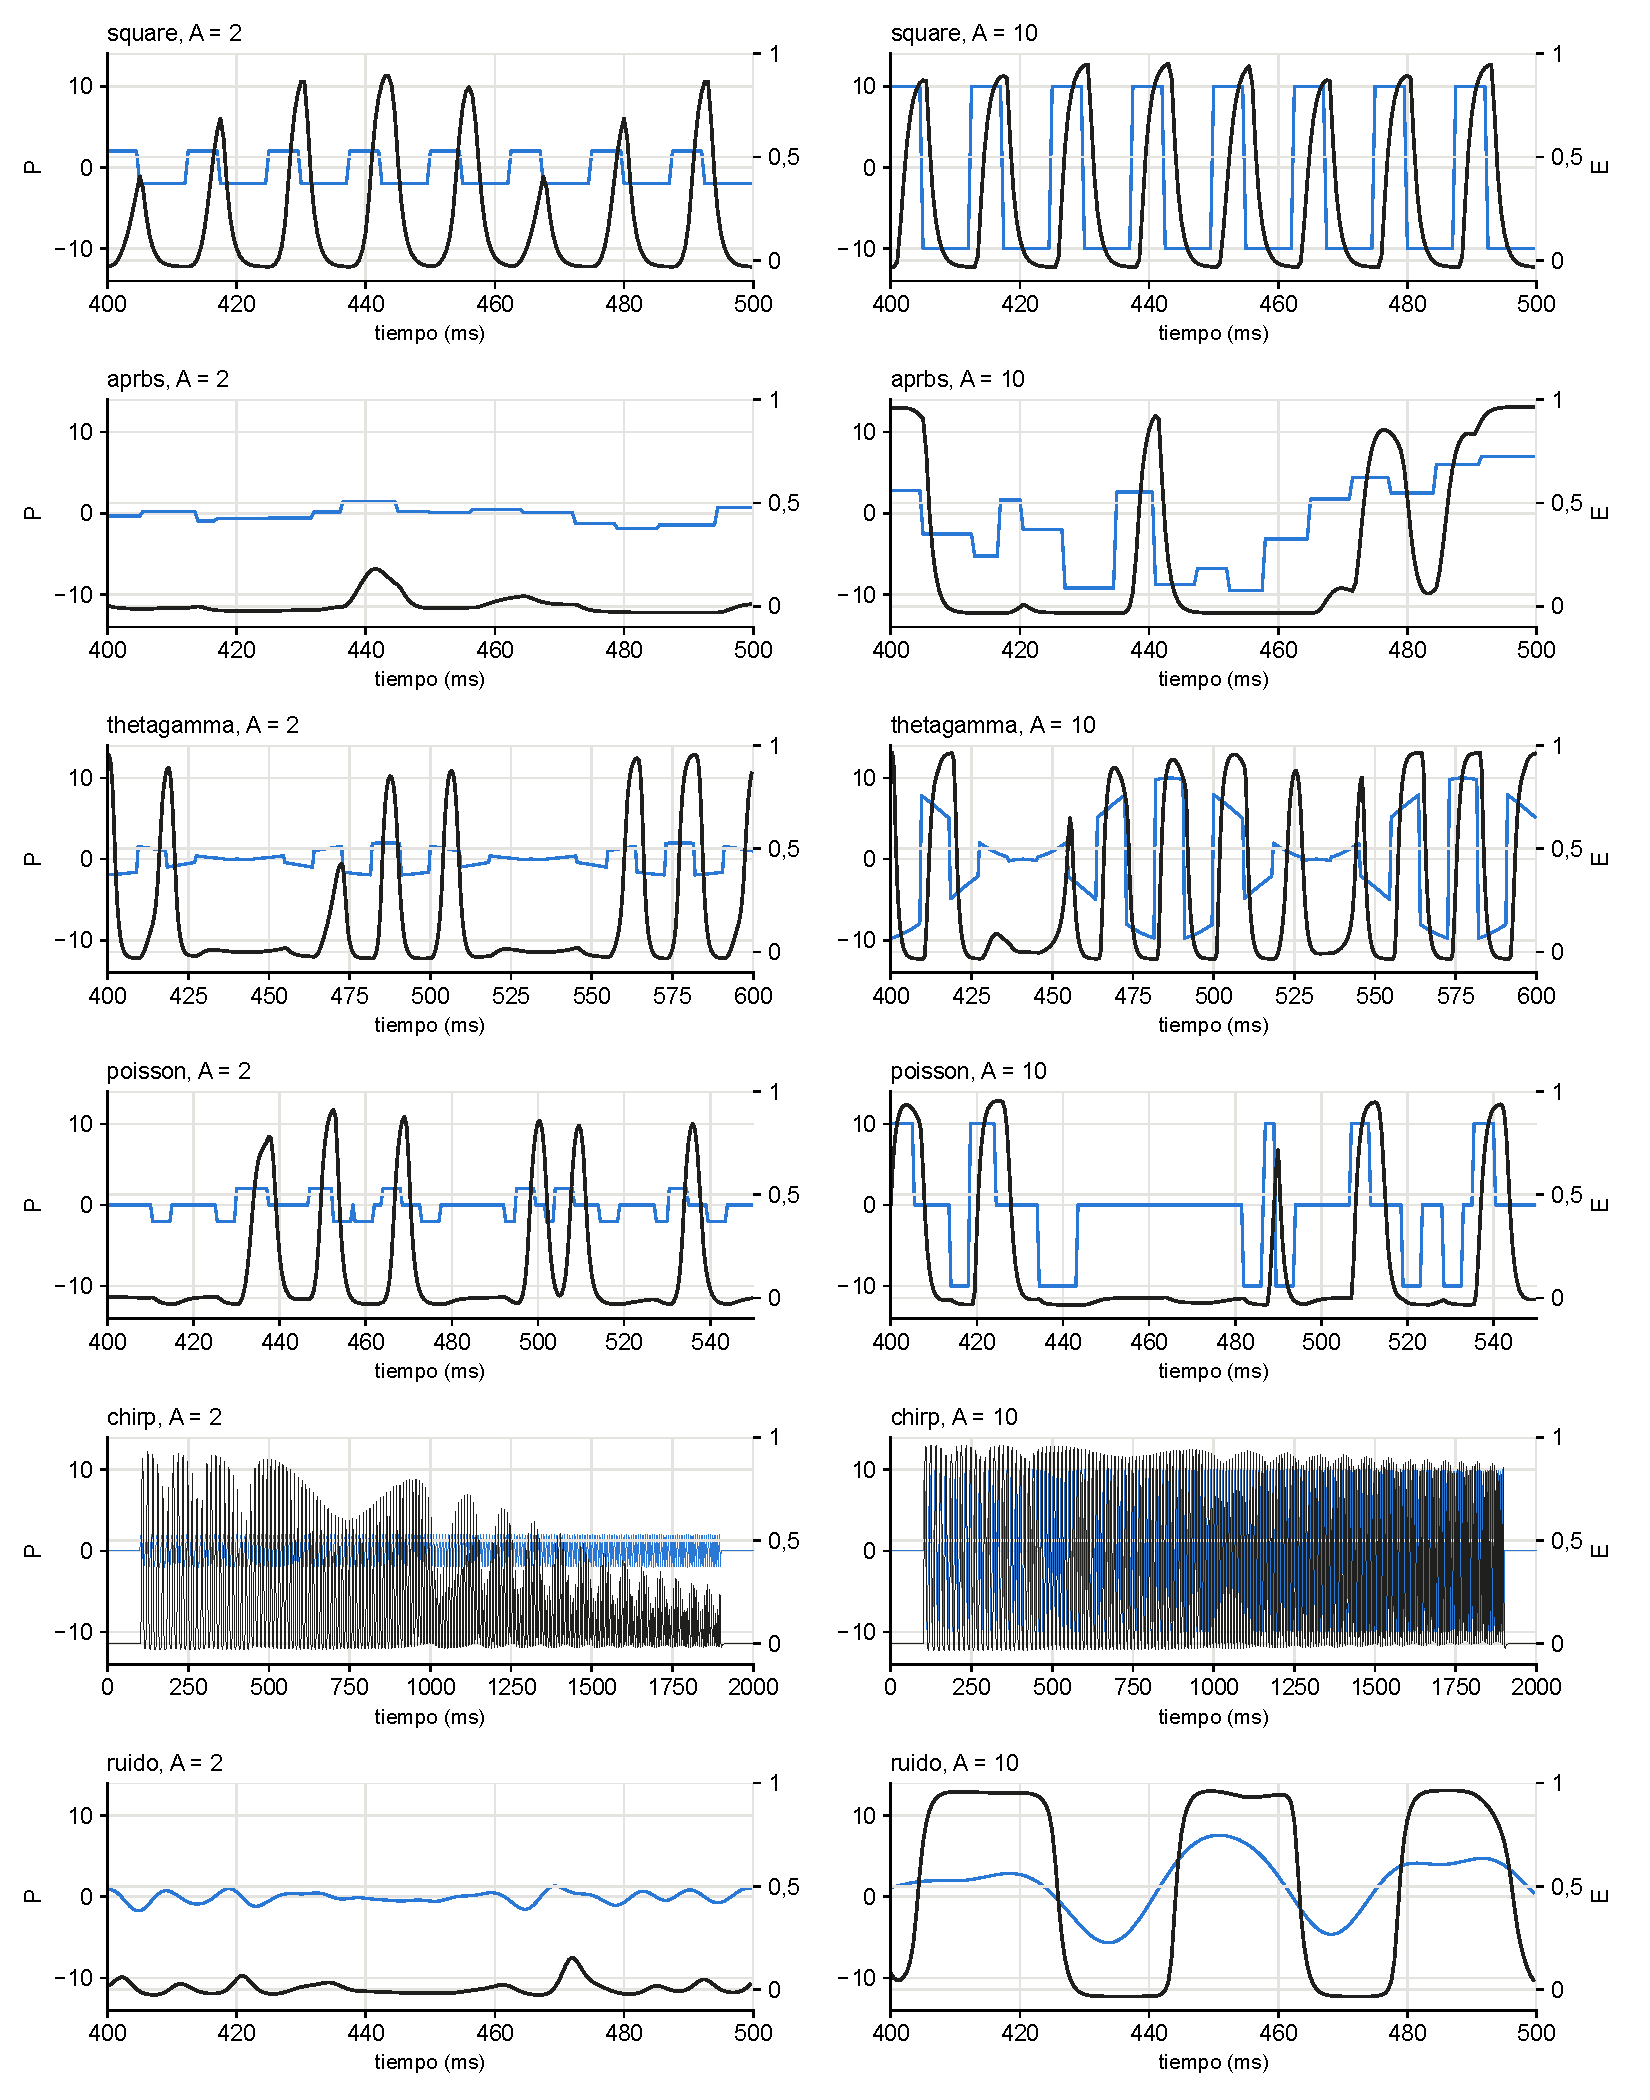
\includegraphics[width=0.95\textwidth]{ejemplos_amplitud.pdf}
\caption{Comando $P$ (azul, eje izquierdo) y actividad $E$ de la planta con actuador (negro, eje derecho) para cada familia de estímulos del régimen de amplitud grande, con amplitud 2 (izquierda) y 10 (derecha), entre 400 y 520~ms.}
\label{fig:ejemplos}
\end{figure}

\subsection{Modelos}

Los modelos con corrección son aditivos,
\begin{equation}
\dot x = \fwc(x, u; \beta) + g_\phi(\xi),
\label{eq:graybox}
\end{equation}
donde $\xi$ es la entrada de la corrección y cambia según la variante. Los diez parámetros se guardan como variables libres $\tilde\beta$ con $\beta = \mathrm{softplus}(\tilde\beta)$, para que sean positivos. La corrección $g_\phi$ es un perceptrón de dos capas ocultas de 32 unidades con tangente hiperbólica, cuya última capa arranca en cero, de modo que al inicio del entrenamiento el modelo coincide con el backbone. El modelo se integra con RK4 de paso $\Delta t$, con el comando retenido durante el paso.

\textbf{White-box.} El backbone \eqref{eq:wc} solo, con los diez parámetros entrenables y $g_\phi \equiv 0$.

\textbf{Corrección agnóstica.} $\xi = (I, E)$. La corrección depende solo del estado actual. Con $g_\phi$ independiente de $u$, el modelo sigue siendo afín en el comando dentro de cada sigmoidea.

\textbf{Historia con comando actual.} $\xi = (I, E, P_k, \dots, P_{k-K+1}, Q_k, \dots, Q_{k-K+1})$, con $K = 10$, o sea 5~ms del comando. El comando actual entra en la sigmoidea y en la red.

\textbf{Historia sin comando actual.} La misma entrada sin $P_k$ ni $Q_k$, con los nueve comandos anteriores. El modelo queda afín en el comando actual.

\textbf{Filtro entrenable.} Una capa lineal sin sesgo resume la historia del comando, $z = A\,h_k$ con $h_k \in \mathbb{R}^{2K}$, $K = 40$ (20~ms) y $A \in \mathbb{R}^{8\times 2K}$, y la red recibe $\xi = (I, E, z)$. Cada fila de $A$ es un filtro FIR sobre los dos comandos, entrenado junto con la red sin forma impuesta.

\textbf{Backbone expandido.} Agrega al white-box la ecuación del mecanismo omitido, con sus parámetros físicos entrenables y sin red. En la planta refractaria agrega el factor $(1 - \hat r_j x_j)$ de \eqref{eq:refrac}, con $\hat r_j$ inicial 0,05. La implementación incluye además una saturación $\tanh(\hat\alpha u)/\hat\alpha$ del comando, que en esta planta terminó en el canal lineal, y suma 13 parámetros. En la planta con actuador aumenta el estado con una copia del filtro,
\begin{equation}
y = (I, E, \hat P, \hat Q)^\top,\qquad \hat\tau\,\dot{\hat P} = P - \hat P,\qquad \hat\tau\,\dot{\hat Q} = Q - \hat Q,\qquad \dot x = \fwc\big(x,\ s(\hat P),\ s(\hat Q);\ \beta\big),
\label{eq:lag}
\end{equation}
con $s(v)$ el recorte en $\pm 1/\hat\alpha$, nivel inicial 10, y 12 parámetros en total. En la línea con tanh, $s(v) = \tanh(\hat\alpha v)/\hat\alpha$. El estado del filtro no se observa. Al inicio de cada ventana se calcula filtrando el comando entero con $\hat\tau$, con la solución exacta del retenedor de orden cero. Este modelo recibe como conocimiento previo el orden del filtro y la forma del recorte.

\textbf{Black-box.} Una Neural ODE sin backbone, $\dot x = g(I, E, P, Q)$, con 64 unidades por capa, y su variante con la historia del comando de 5~ms. Sirven de referencia para separar el aporte del backbone.

\begin{table}[H]
\centering
\footnotesize
\caption{Modelos comparados. «Afín en $u_k$» indica si el comando actual entra solo sumado al argumento de la sigmoidea, que es la condición del despeje cerrado del controlador de \cite{martinez2022ifac}.}
\label{tab:modelos}
\setlength{\tabcolsep}{4pt}
\begin{tabular}{@{}lllcc@{}}
\toprule
modelo & entrada de la red & memoria del comando & afín en $u_k$ & parámetros \\
\midrule
white-box & sin red & no & sí & 10 \\
agnóstica & $I, E$ & no & sí & 1228 \\
historia con comando actual & $I, E$, 5~ms del comando & 10 muestras & no & 1868 \\
historia sin comando actual & $I, E$, 9 comandos anteriores & 9 muestras & sí & 1804 \\
filtro entrenable & $I, E$, 8 canales FIR de 20~ms & 40 muestras & no & 2124 \\
backbone expandido refractario & sin red & no & sí & 13 \\
backbone expandido con actuador & sin red & un polo, $\hat\tau$ & no & 12 \\
black-box & $I, E, P, Q$ & no & no & 4610 \\
\bottomrule
\end{tabular}
\end{table}

\subsection{Entrenamiento}

\textbf{Multiple shooting.} Las trayectorias de entrenamiento se parten en ventanas de 10 muestras (5~ms). Cada ventana arranca del estado observado y se integra con el comando registrado. La pérdida es el error cuadrático medio entre la trayectoria predicha y la observada, sobre todas las ventanas \cite{ribeiro2020,turan2022}.

\textbf{Optimización.} Adam durante 1500 épocas, con tasas de 0,05 para los pesos sinápticos, 0,02 para los demás parámetros físicos y 0,003 para la red, y el gradiente recortado en norma 10. Después, L-BFGS solo sobre los parámetros físicos, salvo en el backbone expandido con actuador y en la black-box. La black-box usa 3000 épocas.

\textbf{Selección por validación.} Cada 100 épocas y al final, el modelo se integra libre sobre los escenarios de validación y se guarda el estado con menor NRMSE de validación. El test no se usa para elegir nada. La agnóstica de la planta refractaria se corrió además con ventanas de 20~ms (40 muestras), y en las tablas se distingue por el largo de la ventana.

\textbf{Arranque.} Las correcciones con red y el backbone expandido con actuador se entrenan dos veces, desde cero (los diez parámetros en 1,0) y desde el white-box (warm start), con el $\bh$ del white-box entrenado sobre los mismos datos y el mismo nivel de ruido. El white-box y la black-box se entrenan solo desde cero. El backbone expandido refractario se entrena solo con warm start, porque desde cero $\hat r_j$ queda trabado en el borde y el modelo colapsa al white-box.

\textbf{Estado inicial entrenable (x0 entrenable).} En una segunda etapa, el modelo parte del checkpoint ya entrenado (parámetros y red) y se libera el estado inicial de cada ventana, $x_0^{(w)}$, con un término de continuidad entre ventanas consecutivas,
\begin{equation}
\mathcal{L} = \frac{1}{N}\sum_{w}\sum_{t}\big\|\hat x^{(w)}_t - x^{(w)}_t\big\|^2 + \lambda \sum_{w}\big\|\hat x^{(w)}_{\text{fin}} - x_0^{(w+1)}\big\|^2,\qquad \lambda = 1,
\end{equation}
siguiendo \cite{turan2022,giampiccolo2024}. En el backbone expandido con actuador se liberan solo los estados iniciales de $I$ y $E$, porque el del filtro sale del comando. En la selección por validación de esta etapa compite también el modelo de partida.

\subsection{Métricas de lazo abierto}

\textbf{NRMSE de corrida libre.} Cada escenario de test se integra entero desde $x(0)$, con el estímulo como única entrada y sin reanclarse a los datos. Por canal, $\mathrm{NRMSE} = 100\cdot\mathrm{RMSE}/(\max - \min)$ de la señal medida, y se promedian $I$ y $E$. En el régimen de amplitud chica se reporta la media sobre los 13 escenarios que interpolan. En el de amplitud grande, la media sobre los 12 escenarios nuevos, salvo que se indique otra cosa. Con ruido, el NRMSE tiene un piso que depende de $\sigma$, y solo se compara dentro de un mismo nivel.

\textbf{Error de los parámetros.} El error relativo medio de los diez parámetros, $100\cdot\frac{1}{10}\sum_j |\bh_j - \beta_j|/\beta_j$.

\textbf{Reconstrucción del término omitido.} La corrección efectiva del modelo es
\[
\hat g = f_{\text{modelo}} - \fwc(x, u; \bh),
\]
evaluada sobre las trayectorias medidas de test. Se compara con $\Delta f$ mediante
\begin{equation}
R^2 = 1 - \frac{\sum_{s}\sum_{t}\big\|\hat g_{s,t} - \Delta f_{s,t}\big\|^2}{\sum_{s}\sum_{t}\big\|\Delta f_{s,t} - \overline{\Delta f}\big\|^2},
\end{equation}
donde $s$ recorre los escenarios de test y $t$ sus 4001 muestras. Un $R^2$ negativo indica que $\hat g$ se aleja de $\Delta f$ más que su media.

Salvo aclaración, los valores de lazo abierto son la media de tres semillas.

\subsection{Lazo cerrado}

\textbf{Controlador.} Se usó el controlador IMC de \cite{martinez2022ifac}, con los parámetros de su archivo original y sin modificaciones. Por población, el controlador integra el error y calcula una acción proporcional-integral,
\begin{equation}
\dot Z_x = r_x - x, \qquad U_x = k_{p,x}(r_x - x) + k_{i,x} Z_x,
\end{equation}
con $k_{p,I} = 10$, $k_{i,I} = 5$ y $k_{p,E} = k_{i,E} = 5$. $U_x$ se recorta al rango de la sigmoidea, y el comando se obtiene invirtiendo la sigmoidea del modelo nominal y restando el acoplamiento,
\begin{equation}
P = \theta_e - \frac{1}{a_e}\ln\!\left(\frac{1}{U_E + k_e} - 1\right) - (w_{EE}E - w_{EI}I),
\end{equation}
y lo mismo para $Q$. No hay cota sobre $P$ ni $Q$ ni anti-windup. Sobre la planta nominal, el lazo cerrado queda $\tau_x \dot x = -x + U_x$. El port a Python se verificó contra las ecuaciones del archivo original integradas con Dormand-Prince, con diferencias máximas de $4\times 10^{-4}$ en $I$.

\textbf{Conexión.} El controlador es el mismo en todas las corridas. Cambia la planta, que es el simulador con la perturbación o un modelo identificado a partir de los datos de ese simulador (Fig.~\ref{fig:lazo}). El lazo se integra con RK4 de paso 0,005~ms, con estado inicial e integradores en cero y mediciones sin ruido. Los modelos con historia guardan el comando aplicado y reciben los valores retenidos a paso de 0,5~ms, como en el entrenamiento.

\begin{figure}[H]
\centering
\begin{tikzpicture}[font=\small,
  caja/.style={draw, rounded corners=2pt, align=center, inner sep=5pt, minimum height=13mm, minimum width=28mm},
  flecha/.style={-{Stealth[length=2.2mm]}, semithick}]
\node[caja] (sim) at (7.2,1.9) {simulador\\con perturbación};
\node[caja] (mod) at (11.4,1.9) {modelo identificado};
\node[caja] (r) at (0,0) {referencias\\$r_I(t)$, $r_E(t)$};
\node[caja] (c) at (3.8,0) {controlador IMC\\parámetros originales};
\node[caja, minimum width=66mm] (pl) at (9.3,0) {planta del lazo\\$(I, E, P, Q) \to (\dot I, \dot E)$};
\draw[flecha] (sim.south) -- (sim.south |- pl.north);
\draw[flecha] (mod.south) -- (mod.south |- pl.north);
\node at ($(sim.east)!0.5!(mod.west)$) {o};
\draw[flecha] (r) -- (c);
\draw[flecha] (c) -- node[above] {$P$, $Q$} (pl);
\draw[flecha] (pl.south) -- ++(0,-0.6) -| node[pos=0.25, below] {$I$, $E$} (c.south);
\end{tikzpicture}
\caption{Esquema del lazo cerrado. El controlador conserva los parámetros de \cite{martinez2022ifac}, y la planta del lazo es el simulador con la perturbación o un modelo identificado a partir de sus datos.}
\label{fig:lazo}
\end{figure}

\textbf{Referencias.} Se usaron cuatro, de dos tipos.

\begin{itemize}[leftmargin=*,itemsep=0.15em]
\item Theta-gamma de 2~s: $r_E = 0{,}3\sin(2\pi f_\gamma t) + 0{,}45$ y $r_I = 0{,}2\sin(2\pi f_\gamma t - 0{,}94) + 0{,}25$, con $f_\gamma = 120$~Hz, mientras la fase de una oscilación theta está a menos de $\pi/4$ de su valle, y $r_E = r_I = 0$ fuera de esos tramos. La theta es ruido blanco filtrado entre 4 y 12~Hz con semilla fija.
\item Gamma continua de 50~ms, con las mismas expresiones de $r_E$ y $r_I$.
\item Theta en rango (8~Hz, 500~ms) y gamma en rango (40~Hz, 250~ms). Son la respuesta del Wilson-Cowan sin perturbación a $P(t) = 1 + 0{,}8\sin(2\pi f t)$ y $Q(t) = 0{,}75 + 0{,}6\sin(2\pi f t - 1)$, y están construidas para que el comando del controlador quede dentro del rango de entrenamiento de amplitud chica. Con el simulador como planta, el comando queda dentro de $[0, 2]$ el 99~\% del tiempo.
\end{itemize}

\textbf{Métricas.} El error de seguimiento es
\begin{equation}
\mathrm{RMSE} = \sqrt{\tfrac{1}{2}\big(\mathrm{RMSE}_E^2 + \mathrm{RMSE}_I^2\big)},\qquad
\mathrm{RMSE}_x = \sqrt{\frac{1}{N - n_0}\sum_{k=n_0}^{N-1}(x_k - r_{x,k})^2},\qquad n_0 = N/5,
\end{equation}
o sea sobre el último 80~\% de la corrida. La distancia entre lazos es la misma expresión con la trayectoria del lazo con el simulador en lugar de la referencia. Siguiendo \cite{gevers2005}, un modelo sirve para el control si su lazo se parece al de la planta, así que la distancia es la métrica principal de lazo cerrado. Los valores son medianas de tres semillas.

\subsection{Tandas de corridas}

\begin{table}[H]
\centering
\small
\caption{Tandas de corridas que sostienen los resultados. Todas con los dos niveles de ruido y, salvo e17 (cinco realizaciones del ruido), con tres semillas en las configuraciones de las tablas.}
\label{tab:tandas}
\begin{tabular}{@{}l>{\raggedright}p{0.26\textwidth}>{\raggedright\arraybackslash}p{0.52\textwidth}@{}}
\toprule
tanda & datos & qué se entrenó \\
\midrule
e16 & amplitud chica, refractaria y actuador con tanh & white-box, agnóstica, historias, filtro entrenable y backbone expandido, desde cero y con warm start \\
e17 & amplitud chica, planta ideal & white-box con estado inicial medido, ventanas de 20~ms y estado inicial entrenable \\
e19 & amplitud chica, refractaria y actuador con tanh & segunda etapa con estado inicial entrenable sobre e16 \\
e20 & amplitud chica, refractaria y actuador con tanh & solo la red, con $\beta$ fijo en el valor verdadero \\
e21 & amplitud chica, actuador con recorte & los modelos de e16 sobre el actuador con recorte \\
e22, e23 & amplitud chica, actuador con recorte & segunda etapa con estado inicial entrenable sobre e21 (redes y backbone expandido) \\
e24 & amplitud chica, las dos plantas & black-box y black-box con historia \\
e25 & amplitud grande, las tres plantas & los modelos de e21 y e16, desde cero y con warm start \\
e26 & amplitud grande & segunda etapa con estado inicial entrenable sobre e25 \\
e27 & amplitud grande & black-box y black-box con historia \\
\bottomrule
\end{tabular}
\end{table}

%=====================================================================
\section{Resultados}
%=====================================================================

\subsection{Lazo abierto con amplitud chica}

\textbf{Planta refractaria.} La Tabla~\ref{tab:refrac_chica} resume los modelos de la planta refractaria. Con $\sigma = 0{,}01$, la agnóstica con warm start y el backbone expandido reprodujeron igual (NRMSE de 2,13 y 2,14) y bajaron el error de $\bh$ del white-box de 10,5 a 3,5 y 2,8~\%. Con la semilla 0, el backbone expandido identificó $\hat r_E = 0{,}098$ y $\hat r_I = 0$ (verdaderos 0,10), y la agnóstica reconstruyó el término omitido con $R^2 = 0{,}78$. Desde cero, la agnóstica reprodujo casi igual (2,28) con 18,3~\% de error de $\bh$ y $R^2 = 0{,}42$. Con $\sigma = 0{,}05$ ninguna corrección se separó del white-box en NRMSE. Las dos black-box reprodujeron entre el white-box y las correcciones con $\sigma = 0{,}01$.

\begin{table}[H]
\centering
\small
\caption{Lazo abierto en la planta refractaria con amplitud chica. NRMSE de los 13 escenarios de test que interpolan (\%), error medio de $\bh$ (\%) y $R^2$ contra el término omitido. Media de tres semillas.}
\label{tab:refrac_chica}
\begin{tabular}{@{}lcccccc@{}}
\toprule
& \multicolumn{3}{c}{$\sigma = 0{,}01$} & \multicolumn{3}{c}{$\sigma = 0{,}05$} \\
\cmidrule(lr){2-4}\cmidrule(l){5-7}
modelo & NRMSE & $\bh$ & $R^2$ & NRMSE & $\bh$ & $R^2$ \\
\midrule
white-box & 3,29 & 10,5 & $-$ & 5,91 & 5,4 & $-$ \\
agnóstica, warm start & 2,13 & 3,5 & 0,78 & 5,66 & 6,9 & 0,74 \\
backbone expandido, warm start & 2,14 & 2,8 & 0,97 & 5,70 & 7,6 & 0,94 \\
black-box & 2,88 & $-$ & $-$ & 5,85 & $-$ & $-$ \\
black-box con historia & 3,20 & $-$ & $-$ & 5,99 & $-$ & $-$ \\
\bottomrule
\end{tabular}
\end{table}

\textbf{Planta con actuador.} La Tabla~\ref{tab:act_chica} resume la planta con actuador y recorte. La agnóstica no mejoró la reproducción del white-box (NRMSE de 7,34 contra 7,28) ni reconstruyó el término omitido ($R^2$ de $-0{,}02$ y $-0{,}12$). Las dos correcciones con el comando actual (historia y filtro entrenable) bajaron el NRMSE de 7,3 a 4,1 y 4,2 con $\sigma = 0{,}01$, con errores de $\bh$ parecidos a los del white-box (18,6 y 18,9~\%) y $R^2$ menores a 0,3. La historia sin comando actual reprodujo como la de 5~ms (4,06), con más error de $\bh$ (28,8~\%) y $R^2 = -0{,}73$. El backbone expandido fue el más preciso y recuperó $\beta$ con 0,42 a 0,46~\% de error y $\hat\tau = 0{,}997$~ms con $\sigma = 0{,}01$. Con $\sigma = 0{,}05$ su error de $\bh$ subió a valores de entre 10,3 y 12,2~\%. Su nivel de recorte quedó en el valor inicial de 10 en todas las corridas, porque los comandos de entrenamiento no superan 2 y el recorte no recibe gradiente. Desde cero, las correcciones con red reprodujeron algo peor y con más error de $\bh$ que con warm start (historia 22,2~\%, filtro entrenable 30,0~\%, historia sin comando actual 36,4~\% y agnóstica 28,3~\%, con $\sigma = 0{,}01$). La black-box con historia reprodujo mejor que todas las correcciones con red con $\sigma = 0{,}01$ (3,47) y quedó a la par con $\sigma = 0{,}05$ (Fig.~\ref{fig:blackbox}).

\begin{table}[H]
\centering
\small
\caption{Lazo abierto en la planta con actuador y recorte con amplitud chica. Mismas métricas que la Tabla~\ref{tab:refrac_chica}.}
\label{tab:act_chica}
\begin{tabular}{@{}lcccccc@{}}
\toprule
& \multicolumn{3}{c}{$\sigma = 0{,}01$} & \multicolumn{3}{c}{$\sigma = 0{,}05$} \\
\cmidrule(lr){2-4}\cmidrule(l){5-7}
modelo & NRMSE & $\bh$ & $R^2$ & NRMSE & $\bh$ & $R^2$ \\
\midrule
white-box & 7,28 & 20,1 & $-$ & 7,90 & 16,6 & $-$ \\
agnóstica, warm start & 7,34 & 17,6 & $-0{,}02$ & 7,90 & 22,1 & $-0{,}12$ \\
historia con comando actual, warm start & 4,07 & 18,6 & 0,17 & 6,24 & 27,4 & 0,27 \\
historia sin comando actual, warm start & 4,06 & 28,8 & $-0{,}73$ & 6,30 & 34,2 & $-0{,}77$ \\
filtro entrenable, warm start & 4,23 & 18,9 & 0,13 & 6,72 & 27,6 & 0,15 \\
backbone expandido, desde cero & 2,26 & 0,42 & 1,00 & 5,87 & 12,2 & 0,98 \\
backbone expandido, warm start & 2,25 & 0,46 & 1,00 & 5,86 & 10,3 & 0,99 \\
black-box & 6,50 & $-$ & $-$ & 7,34 & $-$ & $-$ \\
black-box con historia & 3,47 & $-$ & $-$ & 6,19 & $-$ & $-$ \\
\bottomrule
\end{tabular}
\end{table}

\begin{figure}[H]
\centering
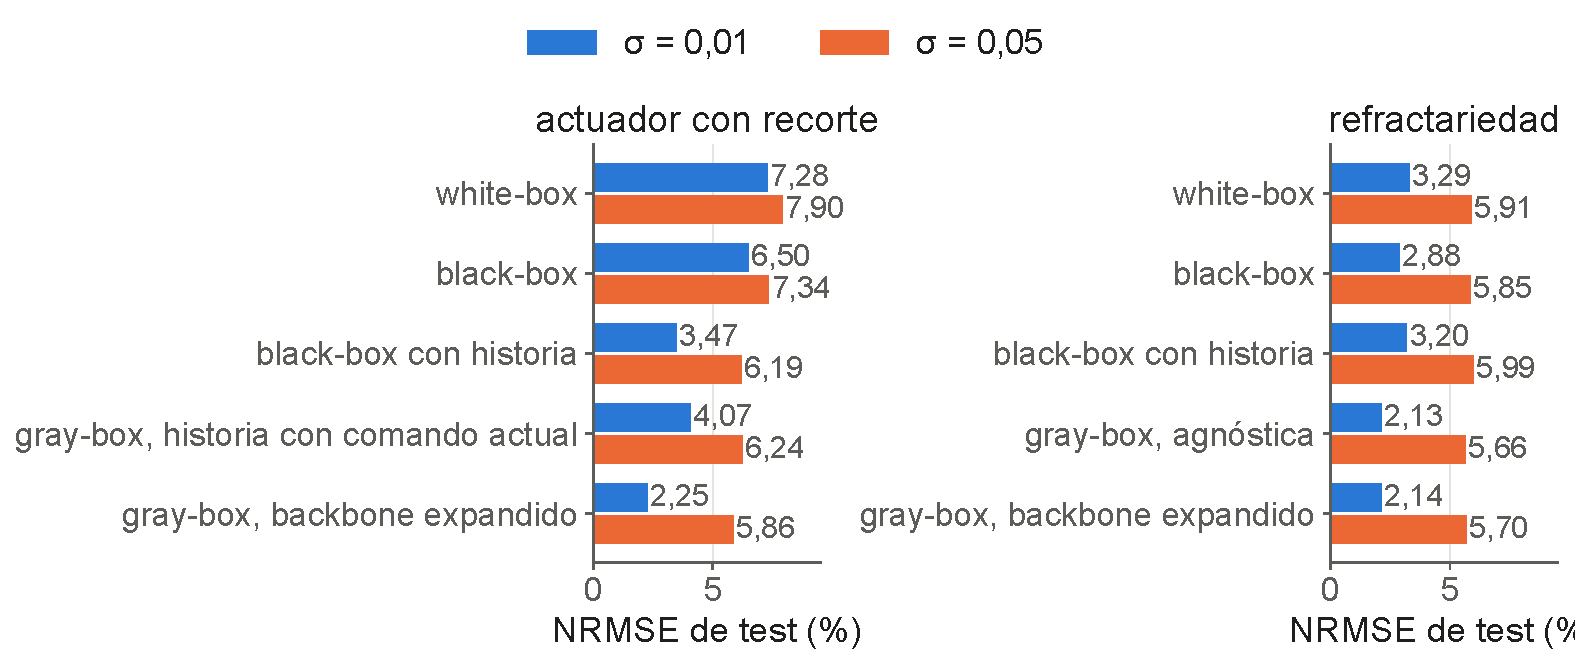
\includegraphics[width=0.85\textwidth]{black_box.pdf}
\caption{NRMSE de test de la black-box $\dot x = g(I, E, P, Q)$ y de la black-box con historia del comando de 5~ms, junto al white-box y a dos modelos gray-box por planta. Amplitud chica, media de tres semillas.}
\label{fig:blackbox}
\end{figure}

Con la saturación $3\tanh(P_f/3)$ en lugar del recorte (e16), las correcciones con red dieron resultados parecidos. El backbone expandido de esa línea tenía la misma forma de saturación que la planta, $\tanh(\hat\alpha v)/\hat\alpha$, pero su nivel no se identificó y $\hat\alpha$ terminó en la cota que anula la saturación. Su error de $\bh$ quedó en 6,7 y 8,7~\% con $\sigma = 0{,}01$ (desde cero y con warm start) y en 12,6 y 14,5~\% con $\sigma = 0{,}05$, porque la compresión por debajo de 3 terminó absorbida en $w_{EE}$, $w_{EI}$ y $a_e$.

\subsection{Capacidad de las redes con los parámetros verdaderos}

Para separar la capacidad de cada red de la interacción con $\bh$, se fijó $\beta$ en el valor verdadero y se entrenó solo la red (e20). Esta tanda se corrió con amplitud chica y con el actuador con tanh. La historia con comando actual reconstruyó el término omitido con $R^2 = 0{,}84$ y el filtro entrenable con 0,74, con $\sigma = 0{,}01$. La historia sin comando actual quedó en 0,19 y la agnóstica del actuador en $-0{,}20$. En la refractaria, la agnóstica llegó a 0,95 (Fig.~\ref{fig:beta_verdadero}). Con $\beta$ libre, la historia sin comando actual reproducía como la de 5~ms porque $\bh$ absorbía parte del término.

\begin{figure}[H]
\centering
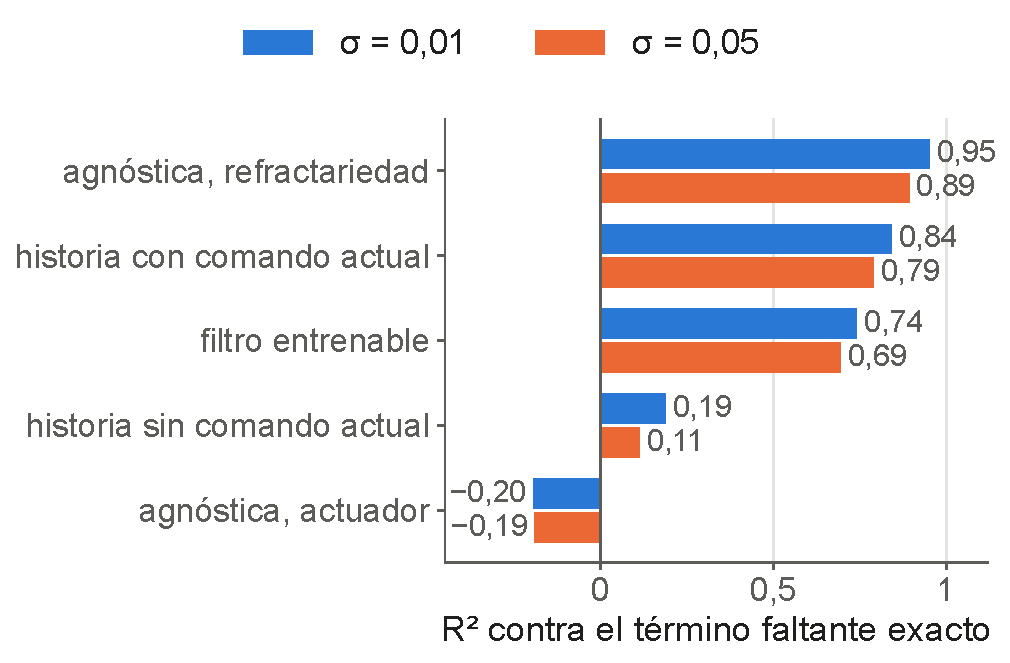
\includegraphics[width=0.6\textwidth]{beta_verdadero_r2.pdf}
\caption{$R^2$ de la red contra el término omitido exacto, con $\beta$ fijo en el valor verdadero y solo la red entrenable (e20). Primera fila, planta refractaria. Las demás, planta con actuador con tanh. Amplitud chica, media de tres semillas.}
\label{fig:beta_verdadero}
\end{figure}

\subsection{Sesgo del entrenamiento por ventanas}

Sobre la planta ideal con $\sigma = 0{,}05$, el white-box entrenado con ventanas de 5~ms que arrancan del estado medido dio 9,8~\% de error medio de parámetros, con los cuatro pesos corridos hacia abajo ($w_{II}$ $-55$~\%). Con ventanas de 20~ms bajó a 4,2~\%, y con el estado inicial entrenable a partir del white-box, a 0,5~\%. Con el estado inicial entrenable desde el arranque ignorante quedó un sesgo de 2 a 4~\%, porque los estados iniciales libres compensan el error de $\bh$.

En la planta refractaria con $\sigma = 0{,}05$, la segunda etapa bajó el error de $\bh$ del backbone expandido de 7,6 a 3,6~\% y el de la agnóstica de 6,9 a 5,6~\% (e19). En la planta con actuador y recorte, el backbone expandido bajó de 0,46 a 0,16~\% con $\sigma = 0{,}01$ y de 10,3 a 1,4~\% con $\sigma = 0{,}05$, con bajas en las tres semillas (de 7,5, 10,3 y 13,0~\% a 1,7, 1,1 y 1,4~\%). Las correcciones con red cambiaron poco (Fig.~\ref{fig:x0}). La historia con comando actual bajó de 27,4 a 23,3~\% con $\sigma = 0{,}05$, y el filtro entrenable subió de 27,6 a 28,3~\%. En el white-box ninguna época de la segunda etapa validó mejor que el modelo de partida.

\begin{figure}[H]
\centering
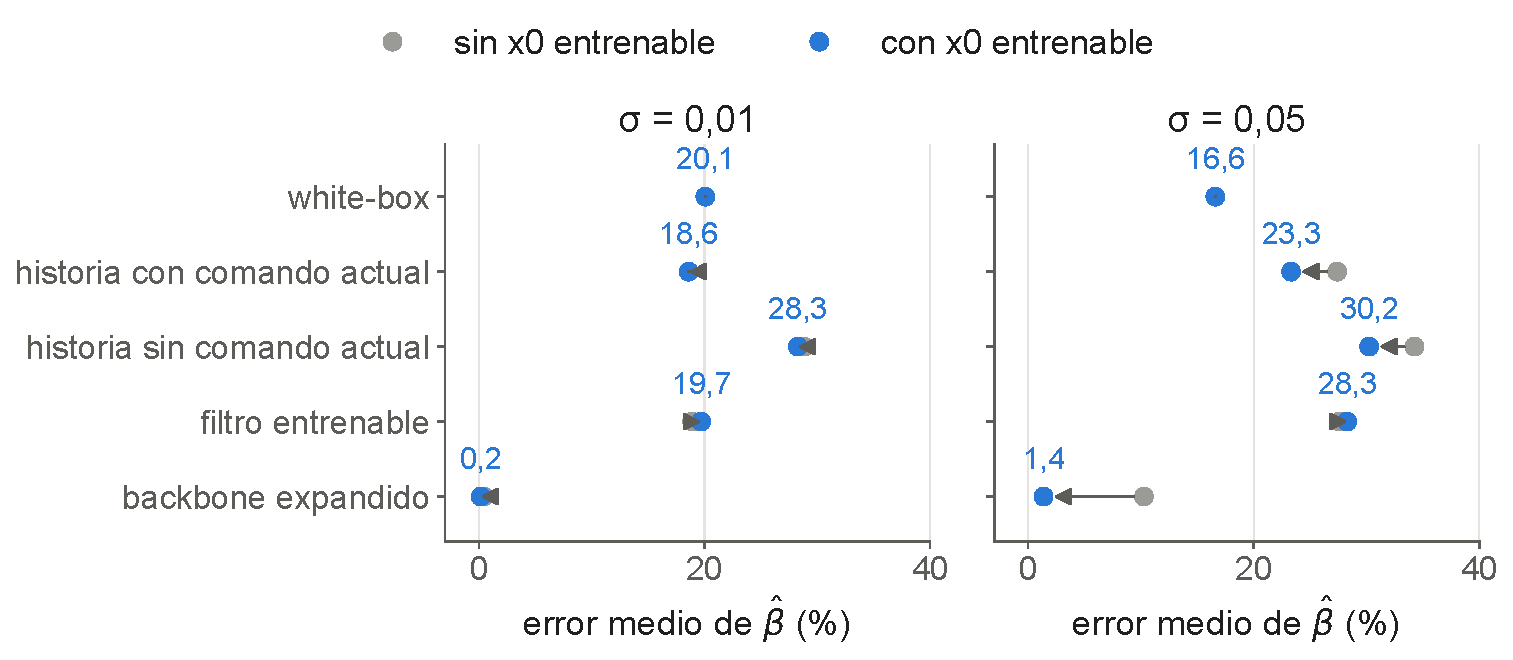
\includegraphics[width=0.85\textwidth]{x0_entrenable_beta.pdf}
\caption{Error medio de $\bh$ antes (gris) y después (azul) de la segunda etapa con estado inicial entrenable, planta con actuador y recorte, amplitud chica. Correcciones con red en e22 y backbone expandido en e23, desde el checkpoint de e21. Media de tres semillas.}
\label{fig:x0}
\end{figure}

\subsection{Lazo cerrado con amplitud chica}
\label{sec:lc_chica}

Con la referencia theta-gamma, el controlador pidió comandos entre $-14$ y $13$ en $P$ y entre $-16$ y $15$ en $Q$, negativos más de la mitad del tiempo. Los modelos entrenados con amplitud chica extrapolan en ese rango.

\textbf{Planta refractaria.} El RMSE de seguimiento del simulador con theta-gamma fue 0,0386, contra 0,0382 de la planta ideal, y los modelos quedaron entre 0,0383 y 0,0401 (media de tres semillas). La perturbación refractaria casi no cambia el lazo cerrado, así que la comparación de lazo cerrado se apoya en la planta con actuador.

\textbf{Planta con actuador.} La Tabla~\ref{tab:lc_chica} muestra el seguimiento y la distancia al lazo con el simulador. El white-box y la agnóstica siguieron la referencia mejor que el propio simulador (0,045 contra 0,057), y sus lazos quedaron a 0,034 del lazo con el simulador. Las correcciones con historia y el filtro entrenable siguieron casi como el simulador o peor (0,059 a 0,077) y quedaron más lejos de su lazo (0,049 a 0,065). El RMSE de seguimiento no ordenó a los modelos según la distancia (Fig.~\ref{fig:rmse_dist}). En las trazas, las correcciones con red oscilaron en los tramos donde la referencia está en reposo (Fig.~\ref{fig:trazas_chica}).

\begin{table}[H]
\centering
\small
\caption{Lazo cerrado sobre la planta con actuador y recorte, modelos entrenados con amplitud chica. RMSE de seguimiento y distancia al lazo con el simulador, mediana de tres semillas, para $\sigma = 0{,}01$ / $0{,}05$ en el entrenamiento del modelo.}
\label{tab:lc_chica}
\setlength{\tabcolsep}{4pt}
\begin{tabular}{@{}lccc@{}}
\toprule
planta en el lazo & RMSE theta-gamma & dist. theta-gamma & dist. gamma 50~ms \\
\midrule
simulador & 0,057 & $-$ & $-$ \\
white-box & 0,045 / 0,043 & 0,034 / 0,035 & 0,061 / 0,062 \\
agnóstica & 0,044 / 0,042 & 0,034 / 0,035 & 0,061 / 0,062 \\
historia con comando actual & 0,059 / 0,063 & 0,049 / 0,054 & 0,068 / 0,066 \\
historia sin comando actual & 0,070 / 0,079 & 0,057 / 0,066 & 0,076 / 0,070 \\
filtro entrenable & 0,077 / 0,078 & 0,065 / 0,071 & 0,067 / 0,067 \\
backbone expandido, nivel entrenado (10) & 0,056 / 0,056 & 0,035 / 0,038 & 0,062 / 0,087 \\
backbone expandido, nivel fijo en 3 & 0,057 / 0,058 & 0,010 / 0,033 & 0,007 / 0,059 \\
\bottomrule
\end{tabular}
\end{table}

\begin{figure}[H]
\centering
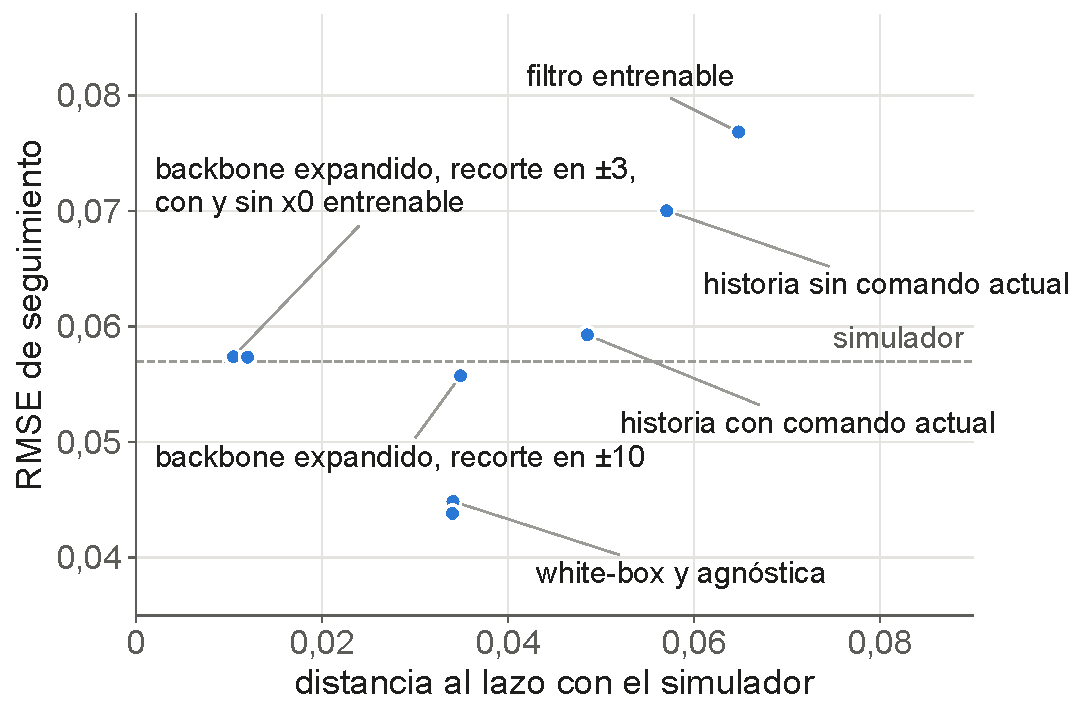
\includegraphics[width=0.55\textwidth]{rmse_vs_distancia.pdf}
\caption{RMSE de seguimiento contra distancia al lazo con el simulador, referencia theta-gamma, planta con actuador y recorte, modelos entrenados con amplitud chica y $\sigma = 0{,}01$. La línea punteada es el RMSE del lazo con el simulador.}
\label{fig:rmse_dist}
\end{figure}

\begin{figure}[H]
\centering
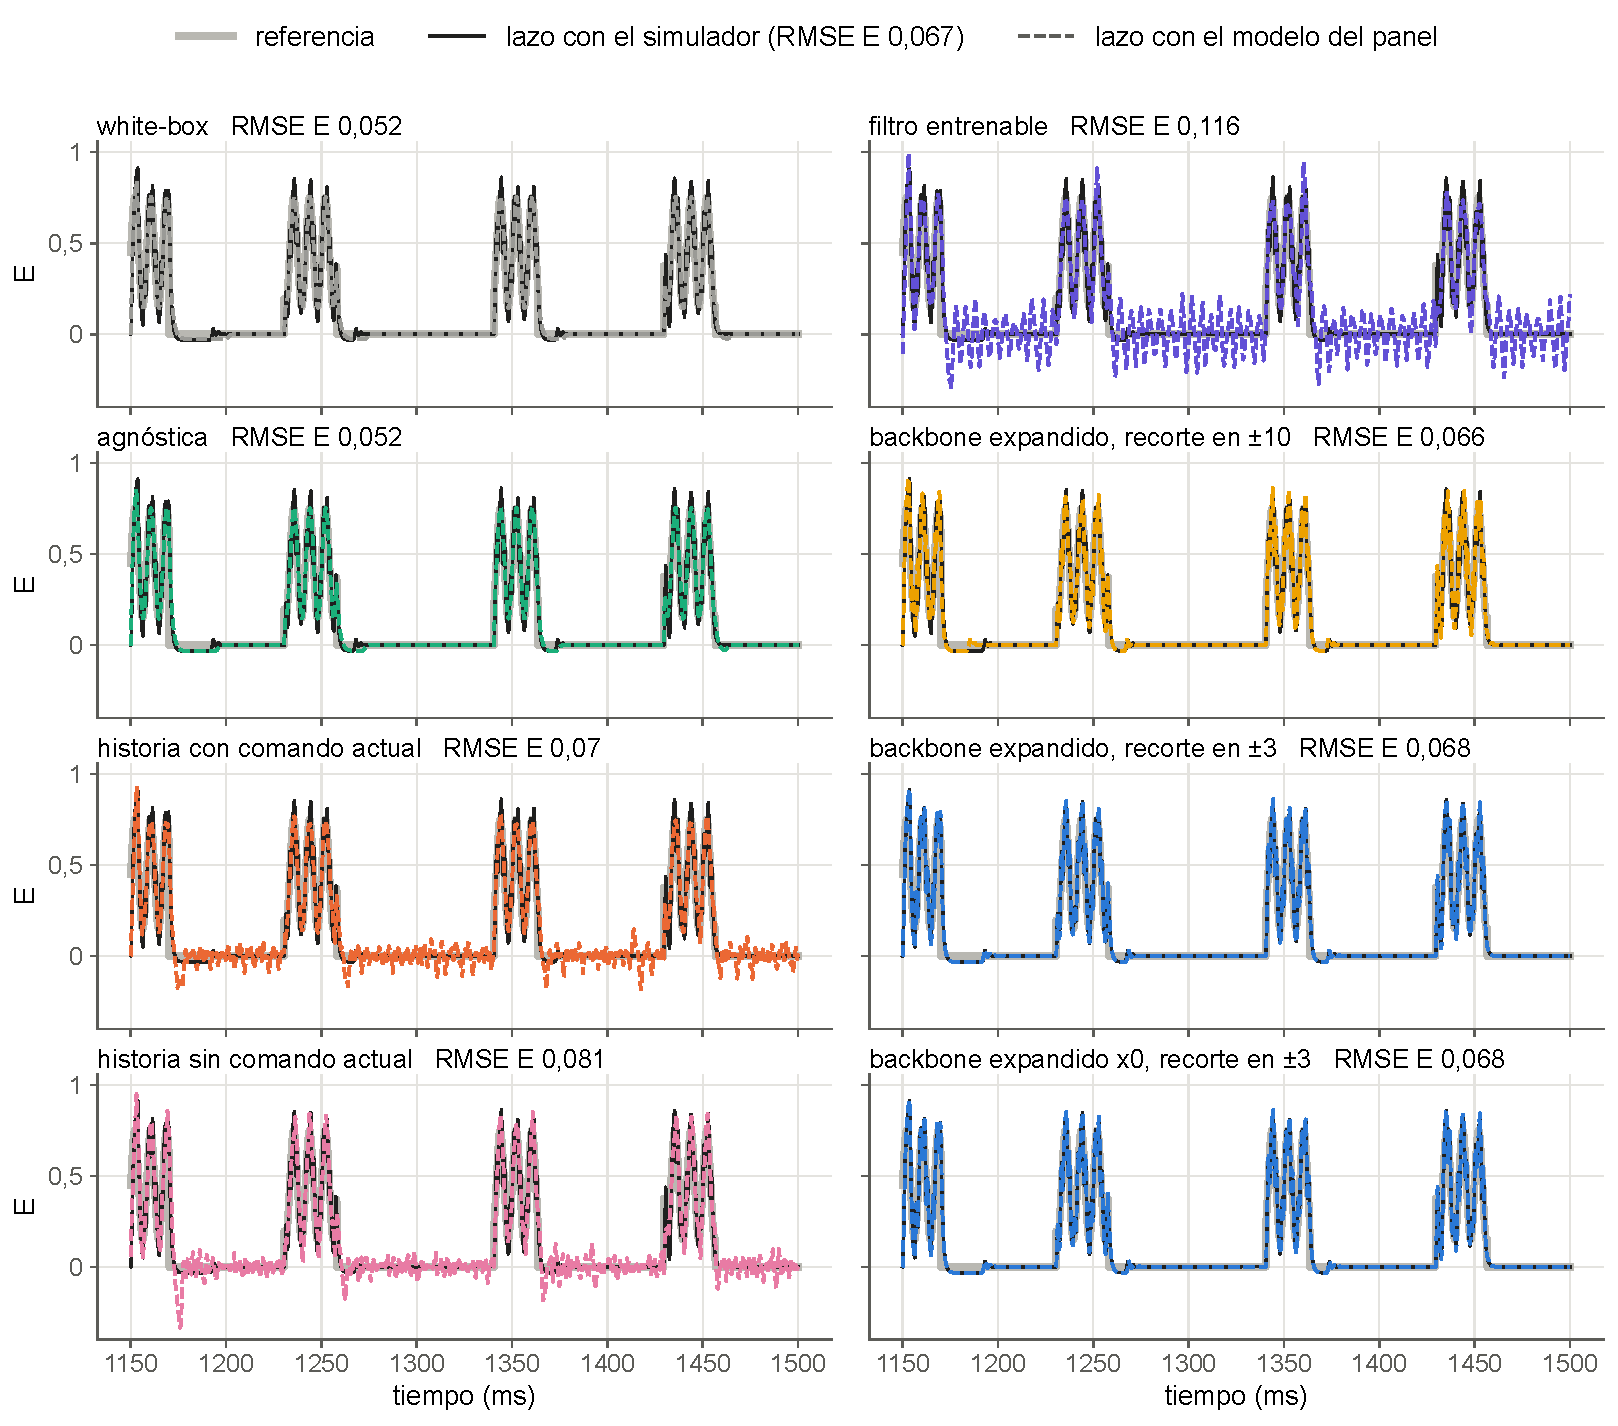
\includegraphics[width=0.95\textwidth]{theta2s_E_chica.pdf}
\caption{Actividad $E$ con la referencia theta-gamma entre 1150 y 1500~ms, planta con actuador y recorte. Gris, referencia. Negro, lazo con el simulador. Discontinua, lazo con el modelo del panel, entrenado con amplitud chica (semilla 0, $\sigma = 0{,}01$). En cada panel, RMSE de $E$ contra la referencia.}
\label{fig:trazas_chica}
\end{figure}

El backbone expandido con el nivel entrenado recortaba en 10, y quedó a la misma distancia que el white-box. Con el nivel fijo en su valor de diseño, 3, y sin reentrenar, su distancia bajó a 0,010 en theta-gamma y a 0,007 en gamma con $\sigma = 0{,}01$. Con $\sigma = 0{,}05$ bajó menos, por el error de $\bh$, y con el estado inicial entrenable de e23 llegó a 0,013 en theta-gamma y 0,019 en gamma (Fig.~\ref{fig:distancias_chica}).

Con las referencias en rango, el backbone expandido reprodujo el lazo del simulador con distancia menor a 0,001 con $\sigma = 0{,}01$, el white-box y la agnóstica quedaron entre 0,001 y 0,003, y las correcciones con historia y el filtro entrenable entre 0,03 y 0,06.

Se repitió además el lazo con un simulador con filtro y sin recorte. Los modelos son los mismos, porque con comandos en $[0, 2]$ los datos de entrenamiento de las dos plantas coinciden. El simulador siguió casi igual que con recorte (0,056 contra 0,057 en theta-gamma). El backbone expandido sin recorte reprodujo ese lazo (0,007 con $\sigma = 0{,}01$), y las correcciones con red quedaron a la misma distancia que con recorte.

\begin{figure}[H]
\centering
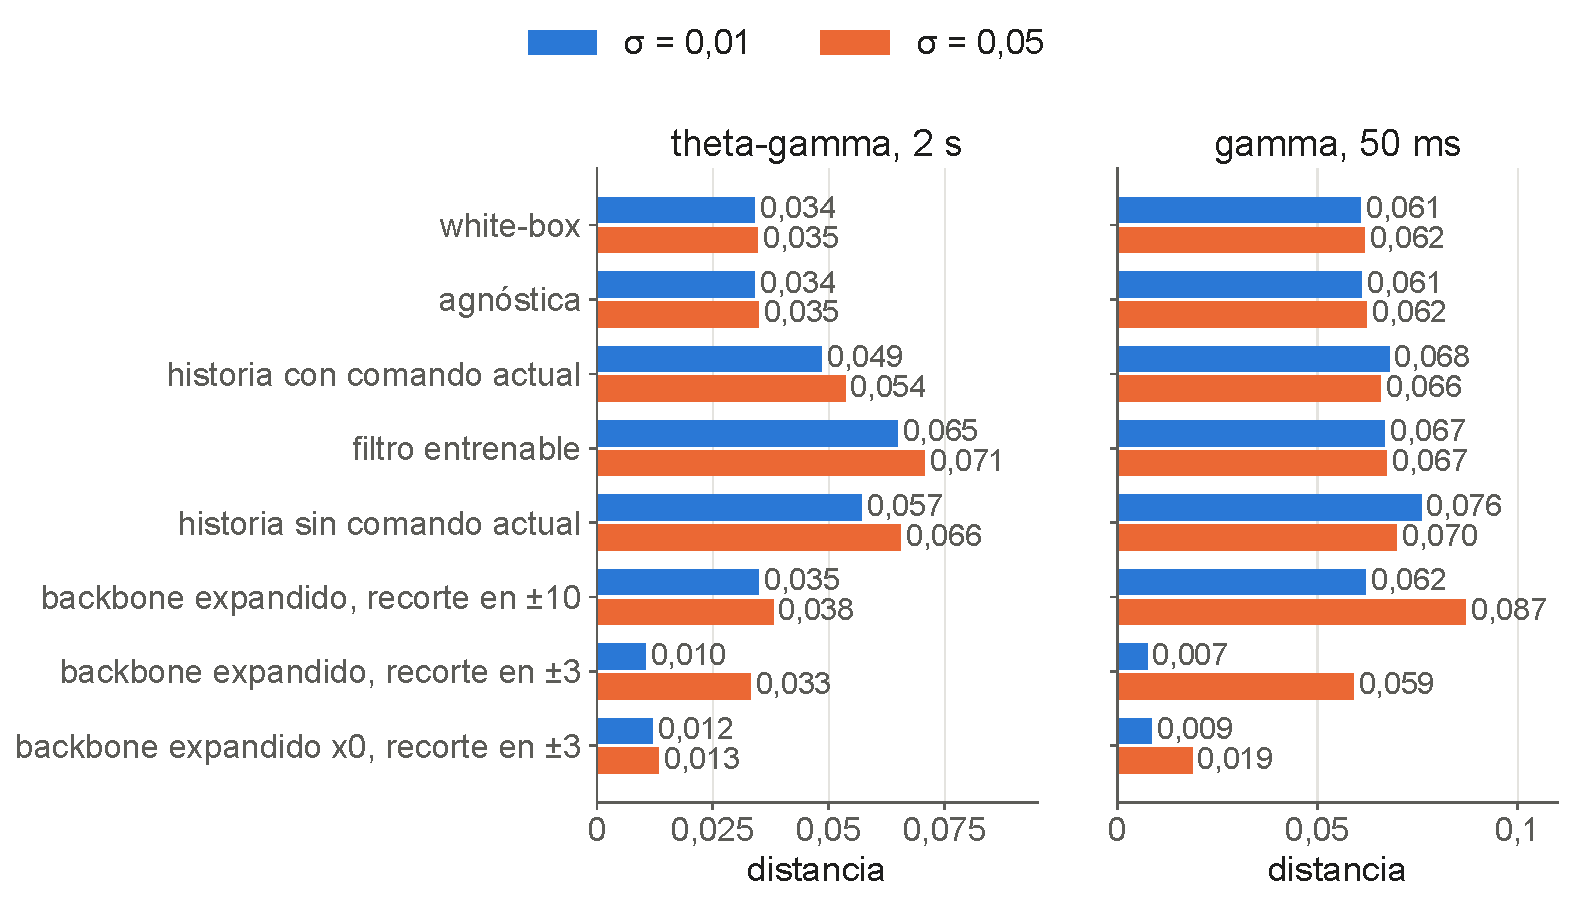
\includegraphics[width=0.75\textwidth]{distancia_lazos.pdf}
\caption{Distancia al lazo con el simulador con actuador y recorte, referencias theta-gamma y gamma de 50~ms, modelos entrenados con amplitud chica. Mediana de tres semillas.}
\label{fig:distancias_chica}
\end{figure}

\subsection{Lazo abierto con amplitud grande}

\textbf{Planta con actuador.} Con comandos de hasta $\pm 12$, el recorte actuó en buena parte del entrenamiento (Tabla~\ref{tab:act_grande}, Fig.~\ref{fig:beta_act_grande}). El backbone expandido identificó $\beta$ con 0,10~\% de error con $\sigma = 0{,}01$ y 0,72~\% con $\sigma = 0{,}05$, que bajó a 0,10~\% con el estado inicial entrenable. En las 18 corridas, $\hat\tau$ salió entre 0,993 y 0,999~ms y el nivel del recorte entre 2,99 y 3,01, partiendo de 10. El white-box llegó a 122~\% de error de $\bh$. Las historias y el filtro entrenable reprodujeron bien los escenarios nuevos (NRMSE de 1,3 a 1,9 con $\sigma = 0{,}01$) con errores de $\bh$ de 110 a 204~\% con warm start y de 42 a 71~\% desde cero, y con $R^2$ entre $-0{,}7$ y 0,25. La agnóstica quedó en 8,1. Entre los modelos sin backbone expandido, la black-box con historia fue la de menor NRMSE (1,09).

\begin{table}[H]
\centering
\small
\caption{Lazo abierto en la planta con actuador y recorte con amplitud grande. Error medio de $\bh$ (\%) y NRMSE en los 12 escenarios de test nuevos. La primera columna es el error de $\bh$ del mismo modelo entrenado con amplitud chica. Con $\sigma = 0{,}05$ el NRMSE tiene un piso de 1,55, que es el del white-box sobre la planta ideal. Media de tres semillas.}
\label{tab:act_grande}
\begin{tabular}{@{}lccccc@{}}
\toprule
& \multicolumn{3}{c}{error de $\bh$ (\%)} & \multicolumn{2}{c}{NRMSE} \\
\cmidrule(lr){2-4}\cmidrule(l){5-6}
modelo & chica, $\sigma$ 0,01 & $\sigma$ 0,01 & $\sigma$ 0,05 & $\sigma$ 0,01 & $\sigma$ 0,05 \\
\midrule
white-box & 20,1 & 121,9 & 121,2 & 10,28 & 9,78 \\
agnóstica, warm start & 17,6 & 44,9 & 46,8 & 8,12 & 7,79 \\
agnóstica, desde cero & 28,3 & 47,4 & 49,4 & 8,31 & 7,94 \\
historia con comando actual, warm start & 18,6 & 117,9 & 114,4 & 1,62 & 2,20 \\
historia con comando actual, desde cero & 22,2 & 42,1 & 41,3 & 1,74 & 2,34 \\
historia sin comando actual, warm start & 28,8 & 204,4 & 210,5 & 1,86 & 2,33 \\
historia sin comando actual, desde cero & 36,4 & 70,7 & 69,7 & 1,89 & 2,47 \\
filtro entrenable, warm start & 18,9 & 109,5 & 109,4 & 1,31 & 2,09 \\
filtro entrenable, desde cero & 30,0 & 43,7 & 44,4 & 1,38 & 2,07 \\
backbone expandido, warm start & 0,46 & 0,10 & 0,72 & 0,37 & 1,60 \\
backbone expandido, desde cero & 0,42 & 0,46 & 0,56 & 0,37 & 1,60 \\
backbone expandido, estado inicial entrenable & 0,16 & 0,10 & 0,10 & 0,37 & 1,59 \\
black-box & $-$ & $-$ & $-$ & 4,71 & 4,69 \\
black-box con historia & $-$ & $-$ & $-$ & 1,09 & 1,94 \\
\bottomrule
\end{tabular}
\end{table}

\begin{figure}[H]
\centering
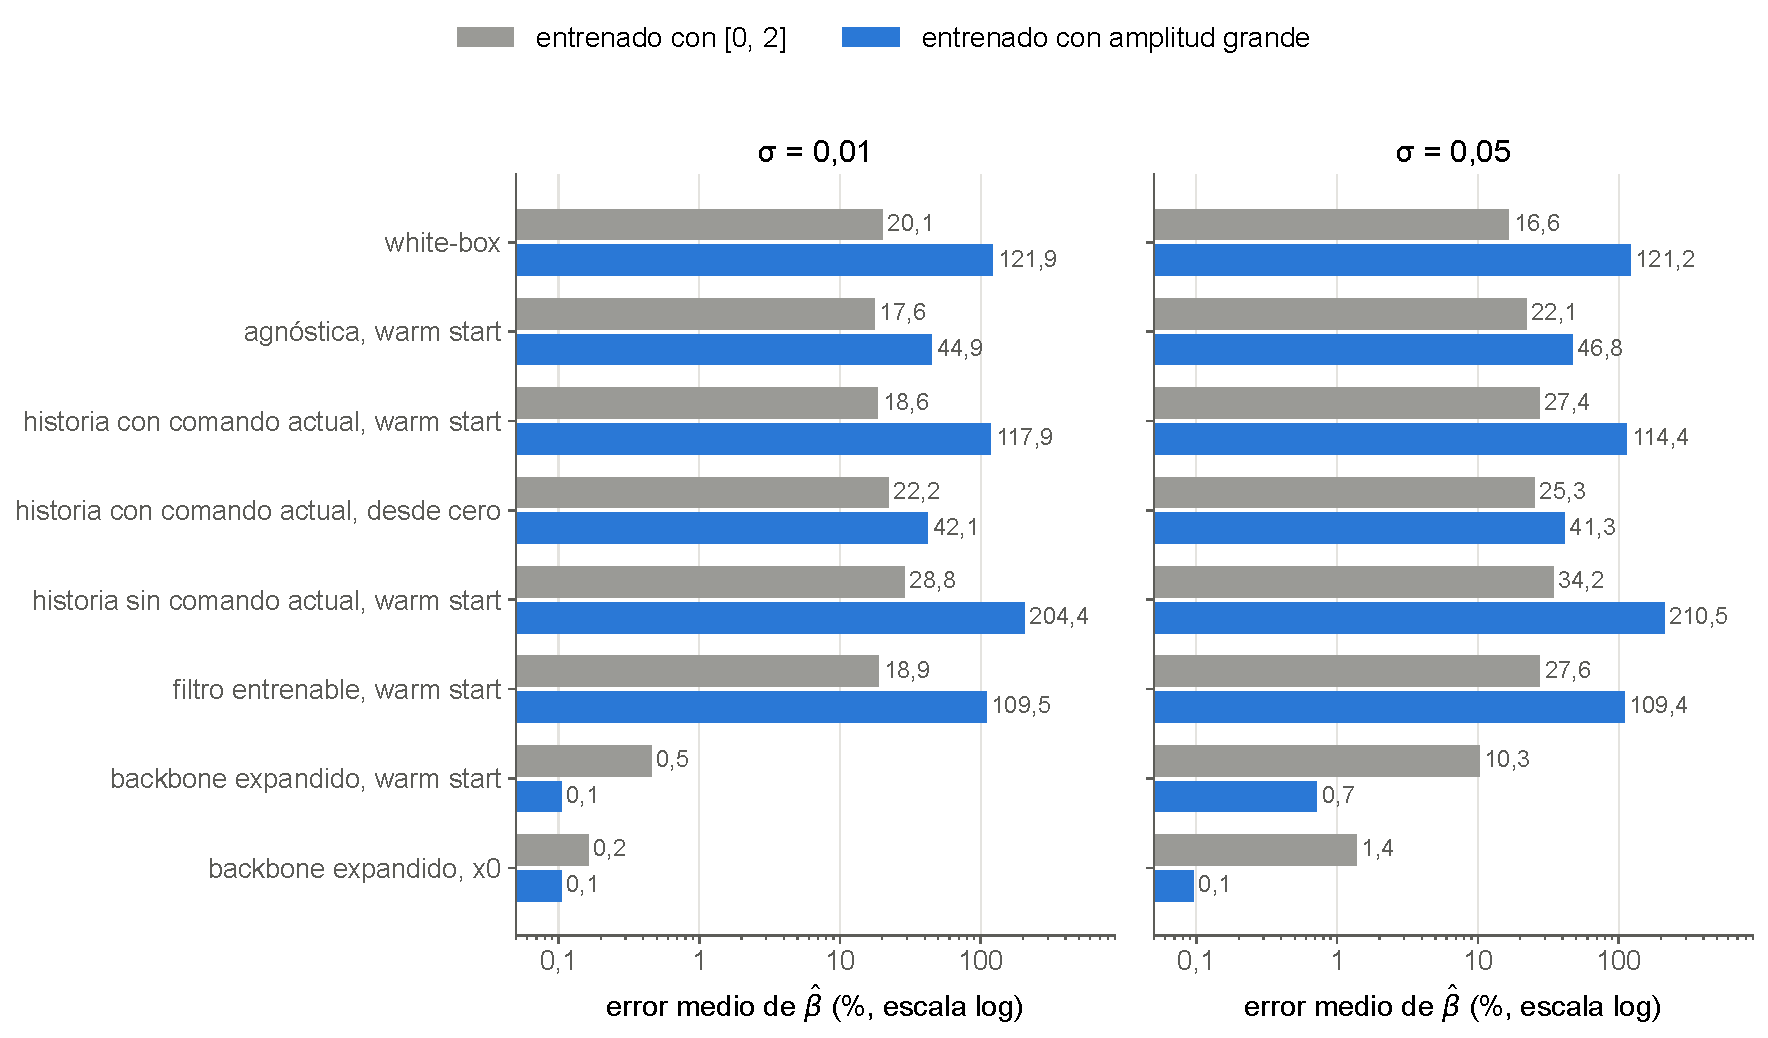
\includegraphics[width=\textwidth]{beta_actuador.pdf}
\caption{Error medio de los diez parámetros en la planta con actuador y recorte, entrenando con amplitud chica (gris) y con amplitud grande (azul), con $\sigma = 0{,}01$ (izquierda) y $\sigma = 0{,}05$ (derecha). Escala logarítmica. Media de tres semillas.}
\label{fig:beta_act_grande}
\end{figure}

La deformación de $\bh$ del white-box tuvo una dirección definida (media de tres semillas, $\sigma = 0{,}01$). Las pendientes $a_e$ y $a_i$ bajaron 36 y 66~\%, los pesos subieron entre 69 y 532~\%, y las constantes de tiempo subieron 70 y 51~\%. En la historia con comando actual desde cero, en cambio, $w_{IE}$ y $w_{II}$ bajaron 66 y 83~\%.

En el test de amplitud chica (los 13 escenarios que interpolan del régimen anterior), el white-box pasó de 7,28 a 23,85 de NRMSE y la agnóstica de 7,34 a 26,93 al entrenarse con amplitud grande. Las correcciones con historia y el filtro entrenable quedaron entre 4,0 y 5,1, y el backbone expandido se mantuvo en 2,25.

\textbf{Planta refractaria.} Todos los modelos con corrección mejoraron la identificación (Tabla~\ref{tab:refrac_grande}). La agnóstica identificó $\beta$ con 1,7~\% de error con warm start y 1,8~\% desde cero, contra 3,5 y 18,3~\% con amplitud chica, y su $R^2$ subió de 0,78 a 0,87. El backbone expandido bajó a 0,24~\%. El white-box pasó de 10,5 a 8,8~\%.

\begin{table}[H]
\centering
\small
\caption{Lazo abierto en la planta refractaria con amplitud grande, y white-box sobre la planta ideal. Mismas métricas que la Tabla~\ref{tab:act_grande}.}
\label{tab:refrac_grande}
\begin{tabular}{@{}lccccc@{}}
\toprule
& \multicolumn{3}{c}{error de $\bh$ (\%)} & \multicolumn{2}{c}{NRMSE} \\
\cmidrule(lr){2-4}\cmidrule(l){5-6}
modelo & chica, $\sigma$ 0,01 & $\sigma$ 0,01 & $\sigma$ 0,05 & $\sigma$ 0,01 & $\sigma$ 0,05 \\
\midrule
white-box & 10,5 & 8,8 & 8,9 & 2,51 & 2,89 \\
agnóstica, ventana de 5~ms, warm start & 3,5 & 1,7 & 2,0 & 0,44 & 1,70 \\
agnóstica, ventana de 5~ms, desde cero & 18,3 & 1,8 & 2,1 & 0,46 & 1,71 \\
agnóstica, ventana de 20~ms, warm start & 4,0 & 1,7 & 1,9 & 0,44 & 1,69 \\
agnóstica, ventana de 20~ms, desde cero & 21,7 & 2,3 & 2,4 & 0,53 & 1,72 \\
backbone expandido, warm start & 2,8 & 0,24 & 0,49 & 0,38 & 1,68 \\
backbone expandido, estado inicial entrenable & 3,0 & 0,26 & 0,28 & 0,38 & 1,67 \\
black-box & $-$ & $-$ & $-$ & 0,60 & 1,75 \\
black-box con historia & $-$ & $-$ & $-$ & 0,83 & 1,87 \\
\midrule
white-box, planta ideal & $-$ & 0,27 & 0,63 & 0,35 & 1,55 \\
\bottomrule
\end{tabular}
\end{table}

\textbf{Planta ideal.} El white-box sobre la planta ideal dio 0,27~\% de error de $\bh$ con $\sigma = 0{,}01$ y 0,63~\% con $\sigma = 0{,}05$, contra 9,8~\% con amplitud chica y $\sigma = 0{,}05$. El estado inicial entrenable cambió poco los resultados de esta tanda, salvo en el backbone expandido con actuador con $\sigma = 0{,}05$.

\subsection{Lazo cerrado con amplitud grande}

La Tabla~\ref{tab:lc_grande} y la Fig.~\ref{fig:dist_grande} comparan la distancia al lazo con el simulador de los modelos entrenados en los dos regímenes. El backbone expandido entrenado con amplitud grande reprodujo el lazo del simulador sin fijar ningún parámetro, con distancias de 0,012 en theta-gamma y 0,008 en gamma con $\sigma = 0{,}01$, y de 0,013 con $\sigma = 0{,}05$. Las correcciones con red quedaron entre 0,037 y 0,111 en theta-gamma y gamma. El filtro entrenable fue el que más cambió, con distancias en rango que bajaron de 0,047 a 0,004. La historia sin comando actual empeoró. El white-box y la agnóstica empeoraron con las referencias en rango (de 0,001 a 0,007 y 0,008 en theta). La black-box entró por primera vez al lazo cerrado y quedó a la distancia del white-box en theta-gamma y gamma (0,033 y 0,064), y cerca del simulador con las referencias en rango (0,002 y 0,004). En la planta refractaria todos los modelos quedaron a 0,007 o menos del lazo con el simulador en las cuatro referencias y con los dos niveles de ruido.

\begin{table}[H]
\centering
\small
\caption{Distancia al lazo con el simulador con actuador y recorte, modelos entrenados con amplitud grande y $\sigma = 0{,}01$. Mediana de tres semillas. Entre paréntesis, el mismo modelo entrenado con amplitud chica. El backbone expandido entrenado con amplitud chica conserva el recorte en $\pm 10$.}
\label{tab:lc_grande}
\begin{tabular}{@{}lcccc@{}}
\toprule
planta en el lazo & theta-gamma & gamma 50~ms & theta en rango & gamma en rango \\
\midrule
white-box & 0,037 (0,034) & 0,068 (0,061) & 0,007 (0,001) & 0,021 (0,003) \\
agnóstica & 0,041 (0,034) & 0,071 (0,061) & 0,008 (0,001) & 0,008 (0,003) \\
historia con comando actual & 0,040 (0,049) & 0,075 (0,068) & 0,020 (0,029) & 0,030 (0,044) \\
historia sin comando actual & 0,061 (0,057) & 0,111 (0,076) & 0,072 (0,035) & 0,061 (0,055) \\
filtro entrenable & 0,037 (0,065) & 0,072 (0,067) & 0,004 (0,047) & 0,003 (0,053) \\
backbone expandido & 0,012 (0,035) & 0,008 (0,062) & 0,000 (0,000) & 0,000 (0,000) \\
black-box & 0,033 & 0,064 & 0,002 & 0,004 \\
black-box con historia & 0,036 & 0,078 & 0,003 & 0,004 \\
\bottomrule
\end{tabular}
\end{table}

\begin{figure}[H]
\centering
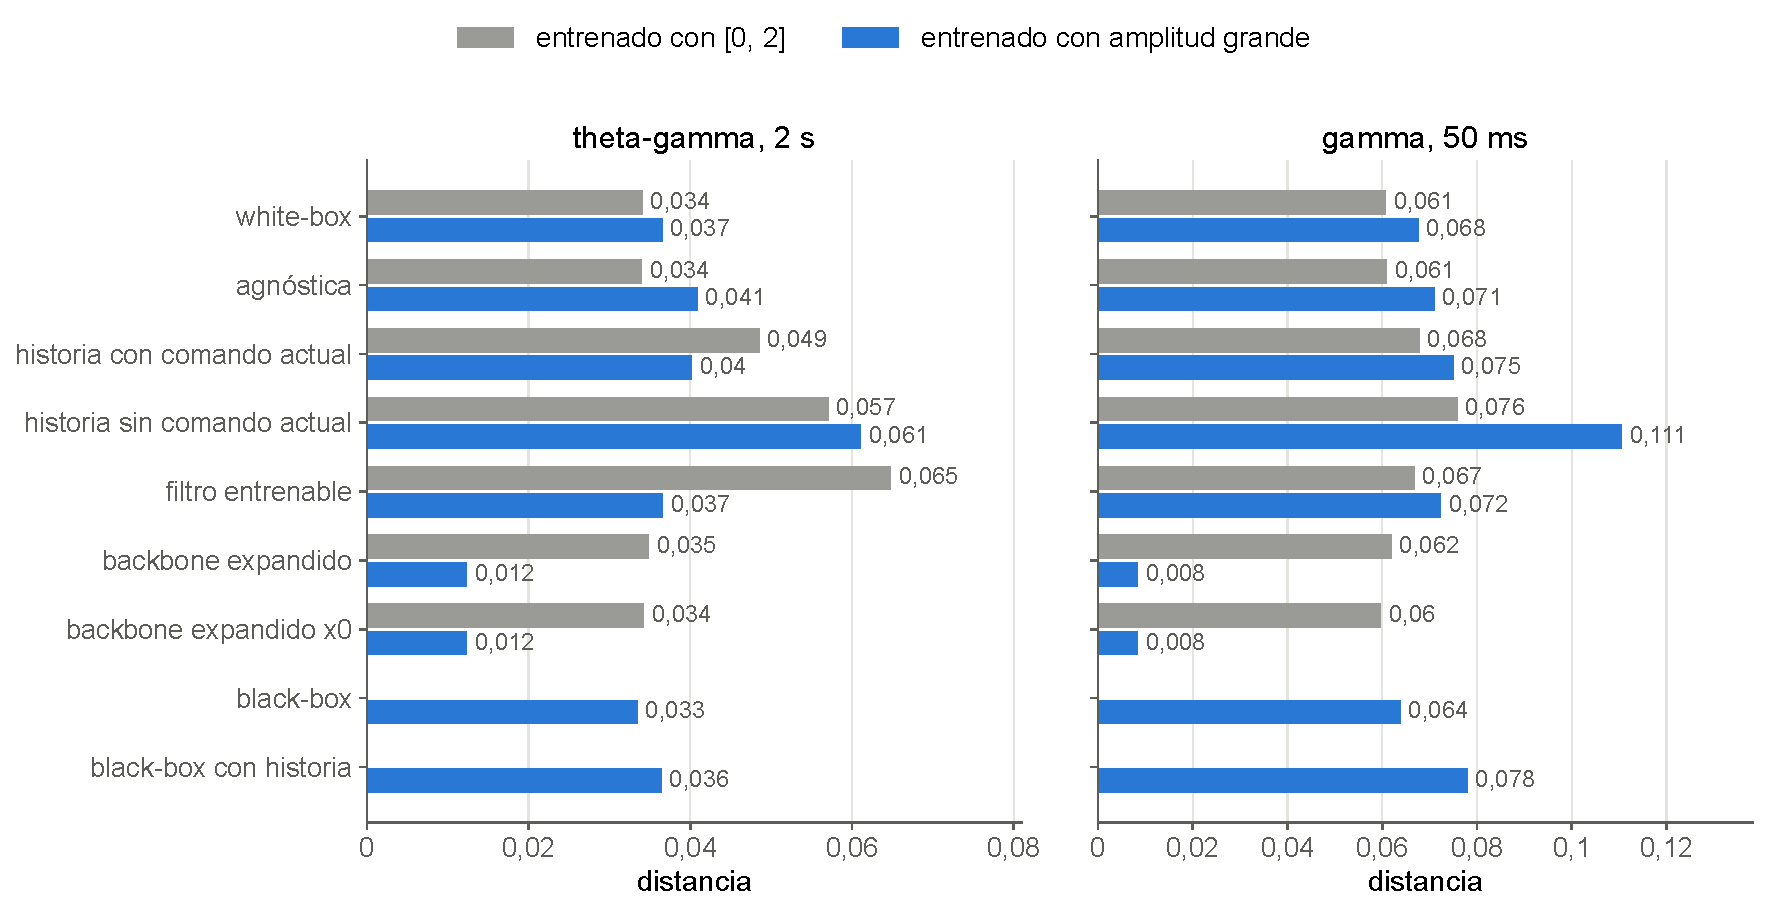
\includegraphics[width=\textwidth]{distancia_lazos_amplitud.pdf}
\caption{Distancia al lazo con el simulador con actuador y recorte, $\sigma = 0{,}01$, para las cuatro referencias, con modelos entrenados con amplitud chica (gris) y con amplitud grande (azul). Mediana de tres semillas.}
\label{fig:dist_grande}
\end{figure}

En las trazas de theta-gamma, el backbone expandido se superpuso al lazo con el simulador (Fig.~\ref{fig:trazas_grande}). El white-box, la agnóstica y la black-box siguieron la forma de las ráfagas y se apartaron en los picos. Las dos historias, el filtro entrenable y la black-box con historia oscilaron entre ráfagas, donde la referencia y el lazo con el simulador están en reposo. Con la gamma continua, el lazo con el simulador quedó atrasado respecto de la referencia por el filtro del actuador, y el backbone expandido reprodujo ese atraso, mientras que la black-box y la agnóstica quedaron en fase con la referencia.

\begin{figure}[H]
\centering
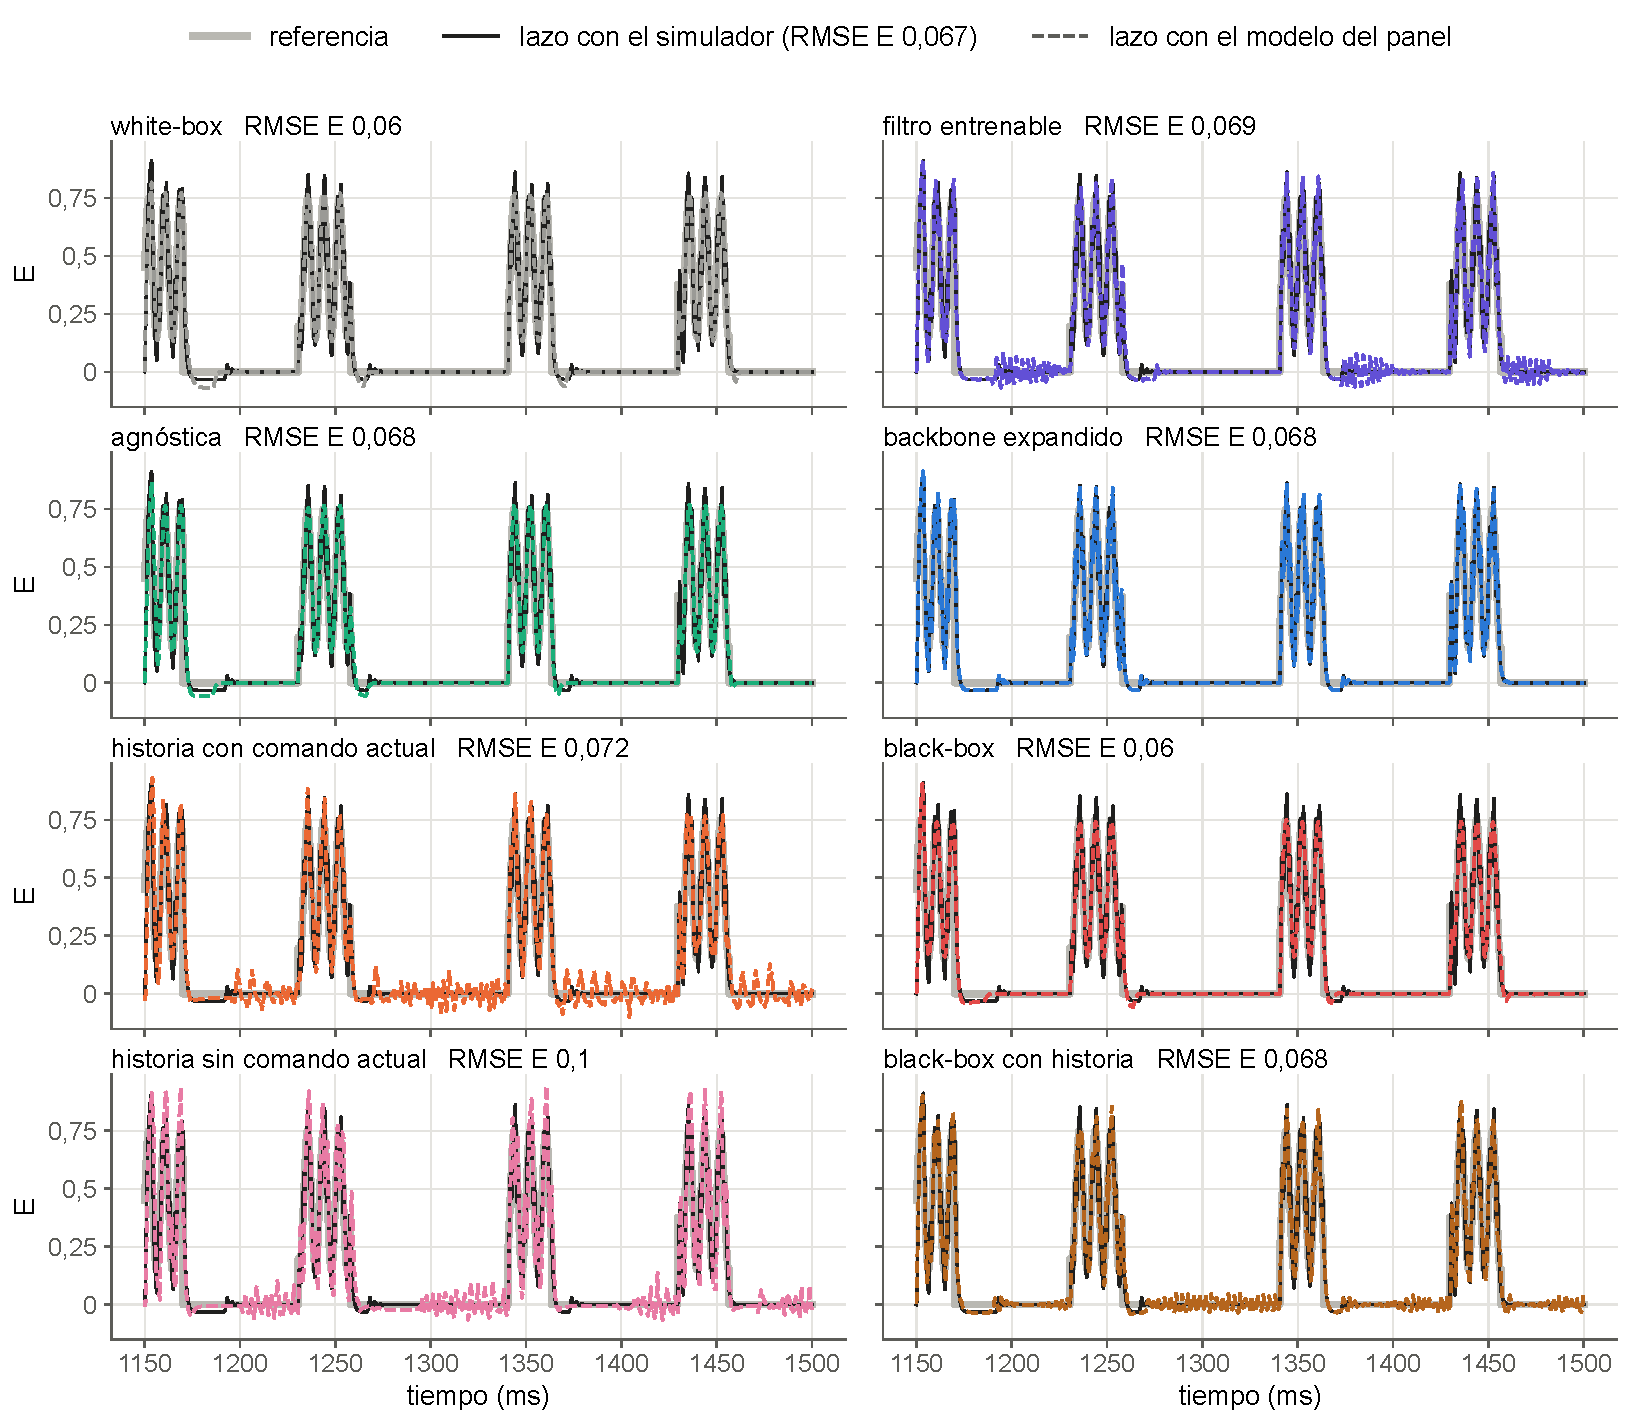
\includegraphics[width=0.95\textwidth]{theta2s_E_amplitud.pdf}
\caption{Actividad $E$ con la referencia theta-gamma entre 1150 y 1500~ms, planta con actuador y recorte. Gris, referencia. Negro, lazo con el simulador. Discontinua, lazo con el modelo del panel, entrenado con amplitud grande (semilla 0, $\sigma = 0{,}01$). En cada panel, RMSE de $E$ contra la referencia.}
\label{fig:trazas_grande}
\end{figure}

%=====================================================================
\section{Discusión}
%=====================================================================

\subsection{La estructura de la corrección y el tipo de física omitida}

En la planta refractaria, una red del estado actual alcanzó para reconstruir el término omitido ($R^2$ de 0,78 con $\beta$ libre y 0,95 con $\beta$ verdadero) y para identificar $\beta$ con warm start. En la planta con actuador, la misma red no mejoró al white-box, y solo las correcciones que reciben el comando actual reconstruyeron parte del término, y solo con $\beta$ fijo en el valor verdadero ($R^2$ de 0,74 a 0,84). Este resultado es compatible con la primera hipótesis, pero las dos plantas difieren también en la magnitud del término omitido, así que no permite separar el efecto de la memoria del efecto de la magnitud.

La historia sin comando actual mostró que la información del instante actual pesa. Con $\beta$ verdadero quedó en $R^2 = 0{,}19$, y con $\beta$ libre reprodujo como la historia completa porque $\bh$ absorbía el término. Es la única corrección con historia que mantiene el modelo afín en el comando, que es la condición para usarla dentro del controlador de \cite{martinez2022ifac}, y en lazo cerrado quedó más lejos del simulador que la historia con comando actual en las cuatro referencias y en los dos regímenes.

Con $\beta$ libre, las correcciones con red de la planta con actuador reprodujeron mejor que el white-box con errores de $\bh$ parecidos o mayores, y con $R^2$ bajos o negativos. La red y los parámetros se repartieron el desajuste de una forma que reproduce la salida sin reconstruir el término. Varias combinaciones de $\bh$ y red reproducen igual de bien, y cada arranque cayó en una distinta. Con amplitud grande, en las historias y el filtro entrenable, el warm start y el arranque desde cero terminaron en errores de 110 a 204~\% y de 42 a 71~\%, con deformaciones en direcciones diferentes. La ventaja del gray-box frente a la black-box, en lazo abierto, quedó en los backbones expandidos y en la refractaria. En el actuador, la black-box con historia reprodujo tan bien como las correcciones con red.

El backbone expandido recibe como conocimiento previo la forma del mecanismo omitido, incluidos el orden del filtro y la forma del recorte. Su desempeño mide lo que aporta la forma correcta, y cuánto se pierde con una forma mal especificada quedó sin medir. La línea con tanh muestra el efecto de un parámetro del mecanismo que los datos no identifican. El nivel de la saturación quedó sin identificar y el error de $\bh$ subió a 6,7 y 8,7~\% con $\sigma = 0{,}01$, contra menos de 0,5~\% con el recorte.

\subsection{El rango de los datos y la identificabilidad}

El nivel del recorte se identificó solo cuando los datos de entrenamiento lo alcanzaron. Con comandos en $[0, 2]$ el recorte no recibía gradiente y quedaba en su valor inicial, y el lazo cerrado necesitaba el nivel de diseño fijado a mano. Con comandos de hasta $\pm 12$ salió entre 2,99 y 3,01 desde un valor inicial de 10, y el modelo reprodujo el lazo sin ajustes.

Ampliar el rango tuvo efectos opuestos según el modelo. En la refractaria, el término omitido crece con la actividad, y con comandos grandes el desvío de $E$ en entrenamiento pasó de 0,17 a 0,34 y la fracción del tiempo con $E > 0{,}3$ de 11 a 29~\%. Un término más grande frente al ruido se separa mejor de $\beta$, y eso coincide con que la agnóstica ya no necesitara warm start. En el actuador, los datos nuevos muestran una saturación que el white-box y las redes no tienen en su estructura, y esos modelos la compensaron deformando $\beta$. El white-box aplanó las sigmoideas y subió los pesos, que es la forma directa de acotar la respuesta, y alargó las constantes de tiempo, compatible con imitar el filtro. En el actuador, con datos más ricos, los modelos sin el recorte identificaron peor.

El warm start, que en la refractaria con amplitud chica fue la condición para que la agnóstica identificara, en el actuador con amplitud grande arrastró la deformación del white-box a las correcciones. Elegir el arranque requiere entonces saber si el white-box de partida está cerca de los parámetros verdaderos, lo que con datos reales no se puede verificar.

\subsection{Lazo abierto y lazo cerrado}

Los resultados de lazo cerrado sostienen la segunda hipótesis. Con amplitud chica, las correcciones con historia y el filtro entrenable redujeron el NRMSE de lazo abierto de 7,3 a 4,1, y sus lazos quedaron más lejos del simulador (0,049 a 0,065) que los del white-box y la agnóstica (0,034). Con amplitud grande reprodujeron en lazo abierto con NRMSE de 1,3 a 1,9 y quedaron a entre 0,037 y 0,111 del lazo con el simulador, con oscilaciones entre ráfagas que el simulador no tiene.

El error de seguimiento tampoco sirvió para elegir modelos. El white-box y la agnóstica siguieron la referencia mejor que la planta, porque el controlador invierte un Wilson-Cowan sin actuador y esos modelos tampoco lo tienen. Seguir la referencia mejor que la planta indica que el modelo se aparta de ella. Por eso la distancia entre lazos se reporta junto al error de seguimiento.

Una explicación posible de la distancia de las redes es que el controlador las lleva a combinaciones de comando y estado que el entrenamiento no cubre, aun con amplitud grande, porque el comando del lazo cambia en cada paso y con una estructura temporal distinta de la de los estímulos. Esta explicación todavía no se puso a prueba.

\subsection{El sesgo del entrenamiento por ventanas}

Arrancar cada ventana del estado medido con ruido sesgó los parámetros del white-box sobre la planta ideal (9,8~\% con $\sigma = 0{,}05$), y el estado inicial entrenable lo corrigió cuando partió de un modelo ya entrenado. En el backbone expandido con actuador, la segunda etapa bajó el error con $\sigma = 0{,}05$ de 10,3 a 1,4~\%, así que su error con ruido alto venía de las condiciones iniciales. En las correcciones con red el error casi no cambió (de 27,4 a 23,3~\% en la que más bajó), lo que ubica su sesgo en la planta con actuador en la estructura del modelo. Con amplitud grande el sesgo casi desapareció (0,63~\% en la planta ideal), porque la respuesta es mucho mayor que el ruido. El método de estado inicial entrenable es práctica conocida \cite{turan2022,giampiccolo2024}, y el aporte de este trabajo está en la medición del sesgo y en su separación del error estructural.

\subsection{Limitaciones}

\begin{itemize}[leftmargin=*,itemsep=0.25em]
\item Todos los datos son sintéticos. El ruido de medición es blanco y más limpio que el de registros reales, y no hay ruido de proceso ni actividad espontánea.
\item Las perturbaciones son de diseño. El filtro de 1~ms es más rápido que la channelrodopsina-2, cuyo $\tau_{\text{off}}$ va de 11 a 14~ms \cite{williams2013}, y el nivel de recorte en 3 se eligió por dificultad. Una perturbación por vez.
\item Los comandos bipolares suponen una actuación capaz de excitar e inhibir cada población. Con una sola opsina excitatoria, los comandos negativos no se pueden realizar.
\item Un solo controlador, sin cota sobre el comando ni anti-windup, con mediciones sin ruido en el lazo cerrado.
\item En lazo cerrado, la planta refractaria casi no se distingue de la ideal, y las conclusiones de lazo cerrado se apoyan en la planta con actuador.
\item La prueba con $\beta$ verdadero (e20) se corrió con amplitud chica y, en el actuador, con la saturación tanh. Las corridas de e19 en el actuador también usaron la tanh.
\item La agnóstica de la planta con actuador con tanh tiene una sola semilla en e16. Con tres semillas, las diferencias menores a algunas décimas de NRMSE no se pueden separar de la variación entre semillas.
\item El backbone expandido recibe la forma correcta del mecanismo omitido.
\end{itemize}

%=====================================================================
\section{Conclusiones}
%=====================================================================

\begin{itemize}[leftmargin=*,itemsep=0.35em]
\item En la planta refractaria, una corrección agnóstica del estado reconstruyó el término omitido e identificó los parámetros del backbone, con warm start en amplitud chica (3,5~\%) y con cualquier arranque en amplitud grande (1,7 a 1,8~\%).
\item En la planta con actuador, solo el backbone expandido recuperó los parámetros (0,1 a 0,5~\% con $\sigma = 0{,}01$), y con comandos que alcanzan el recorte identificó también el nivel de saturación. Las correcciones con historia del comando y con filtro entrenable reprodujeron en lazo abierto con parámetros alejados de los verdaderos (errores de 18,6 a 210~\%) y sin reconstruir el término omitido.
\item Sin el comando actual, una red con historia del comando no reconstruyó el término omitido del actuador, aun con los parámetros verdaderos ($R^2 = 0{,}19$).
\item La precisión en lazo abierto no ordenó a los modelos para el control. Con amplitud chica, las correcciones con red reprodujeron mejor que el white-box y quedaron más lejos del lazo de la planta. Con amplitud grande quedaron a una distancia parecida a la del white-box o mayor. El error de seguimiento favoreció a modelos que se parecen menos a la planta. La distancia entre el lazo con el modelo y el lazo con la planta es la métrica que separó a los modelos.
\item El backbone expandido con actuador reprodujo el lazo de la planta con referencias en rango, y fuera de rango cuando el nivel del recorte se identificó con datos de amplitud grande. Con amplitud chica y el nivel fijado en el valor de diseño lo reprodujo con $\sigma = 0{,}01$, y con $\sigma = 0{,}05$ hizo falta además el estado inicial entrenable.
\item Con ruido de medición, arrancar las ventanas del estado medido sesgó los parámetros. Un estado inicial entrenable, a partir de un modelo ya entrenado, corrigió ese sesgo en el white-box sobre la planta ideal y en el backbone expandido con actuador, y lo redujo a la mitad en el backbone expandido refractario con $\sigma = 0{,}05$. En las correcciones con red de la planta con actuador el error de los parámetros casi no cambió, lo que indica un origen estructural.
\item En la planta con actuador, ampliar el rango de los comandos mejoró la identificación del backbone expandido y empeoró la de los modelos sin el recorte en su estructura. En la planta refractaria mejoró la de todos los modelos.
\end{itemize}

%=====================================================================
\section{Trabajo futuro}
%=====================================================================

\begin{itemize}[leftmargin=*,itemsep=0.25em]
\item Repetir la prueba con $\beta$ verdadero y solo la red entrenable sobre los datos de amplitud grande (e28, 30 corridas, preparada), para separar la capacidad de cada red de la identificabilidad entre $\beta$ y la red cuando el recorte actúa.
\item Evaluar las correcciones con red en lazo abierto con el comando registrado del lazo con el simulador, para distinguir si su distancia en lazo cerrado depende de la región del espacio de estado y comando o de la realimentación.
\item La línea realista del actuador, con constantes de ChR2, filtro asimétrico y el modelo de cuatro estados de \cite{williams2013}.
\item La planta con las dos perturbaciones juntas.
\item Backbones expandidos con la forma del mecanismo mal especificada, y comparación con un estado aumentado genérico \cite{dupont2019} y con un codificador del estado inicial \cite{beintema2021}.
\item Usar la historia sin comando actual dentro del controlador, aprovechando que el modelo queda afín en el comando, o controladores que no invierten el modelo, como el control predictivo.
\item Ruido en el lazo cerrado y, en una etapa posterior, datos reales.
\end{itemize}

\printbibliography[title={Referencias}]

\appendix
%=====================================================================
\section{Parámetros verdaderos e identificados}
\label{ap:parametros}
%=====================================================================

\begin{table}[H]
\centering
\small
\caption{Parámetros verdaderos del backbone y valores identificados con amplitud chica, $\sigma = 0{,}01$, semilla 0, para la planta refractaria y la planta con actuador con tanh (e16).}
\begin{tabular}{@{}lcccccccccc@{}}
\toprule
& $w_{EE}$ & $w_{EI}$ & $w_{IE}$ & $w_{II}$ & $\tau_e$ & $\tau_i$ & $a_e$ & $a_i$ & $\theta_e$ & $\theta_i$ \\
\midrule
verdaderos & 6,40 & 4,80 & 6,00 & 1,20 & 1,00 & 2,00 & 1,20 & 1,00 & 2,80 & 4,00 \\
\midrule
refractaria, white-box & 5,82 & 4,90 & 6,19 & 1,89 & 1,12 & 2,06 & 1,28 & 1,05 & 2,64 & 3,98 \\
refractaria, agnóstica & 6,20 & 4,69 & 6,16 & 1,32 & 1,08 & 2,04 & 1,24 & 0,98 & 2,69 & 4,01 \\
refractaria, backbone exp. & 6,33 & 4,77 & 6,06 & 1,45 & 1,01 & 2,02 & 1,21 & 0,98 & 2,78 & 4,02 \\
actuador, white-box & 8,21 & 7,30 & 6,96 & 2,05 & 1,41 & 2,36 & 1,14 & 0,91 & 3,03 & 4,24 \\
actuador, historia & 9,43 & 7,15 & 6,99 & 0,94 & 1,21 & 1,98 & 0,91 & 0,79 & 3,56 & 4,84 \\
actuador, backbone exp. & 7,46 & 5,51 & 6,46 & 1,36 & 0,98 & 2,00 & 1,01 & 0,93 & 3,13 & 4,25 \\
\bottomrule
\end{tabular}
\end{table}

Perturbaciones: $r = 0{,}10$ en la planta refractaria; $\tau = 1$~ms y recorte en $\pm 3$ en la planta con actuador. Ganancias del controlador: $k_{p,I} = 10$, $k_{i,I} = 5$, $k_{p,E} = 5$, $k_{i,E} = 5$.

%=====================================================================
\section{Detalles de entrenamiento}
%=====================================================================

\begin{table}[H]
\centering
\small
\begin{tabular}{@{}l>{\raggedright\arraybackslash}p{0.62\textwidth}@{}}
\toprule
ventana de multiple shooting & 10 muestras (5~ms); 40 muestras (20~ms) en la agnóstica de 20~ms \\
optimizador & Adam, 1500 épocas (3000 en la black-box), luego L-BFGS sobre $\beta$ (salvo backbone expandido con actuador y black-box) \\
tasas de aprendizaje & 0,05 (pesos), 0,02 (demás parámetros físicos), 0,003 (red) \\
recorte del gradiente & norma 10 \\
red de corrección & 2 capas ocultas de 32 unidades, tanh, última capa inicializada en cero \\
red black-box & 2 capas ocultas de 64 unidades, tanh \\
selección & menor NRMSE de validación, evaluado cada 100 épocas y al final \\
arranque desde cero & los diez parámetros en 1,0 \\
backbone expandido & $\hat r$ inicial 0,05; $\hat\tau \geq 0{,}3$~ms; nivel del recorte inicial 10 \\
segunda etapa & estado inicial por ventana entrenable, continuidad con $\lambda = 1$ \\
integración & RK4 con el comando retenido, $\Delta t = 0{,}5$~ms (modelos) y 0,005~ms (lazo cerrado) \\
\bottomrule
\end{tabular}
\end{table}

\end{document}
